% TODO
%
% opisać rozwiązanie
% bibliografia

% stopień schubigera
% ?podział na rozdziały

% poprawić conclusions/further works
% dopisać ostatni rozdział
% sprawdzić co robi skalowanie
% dodać przywracanie ze spania
% 


% 
% poradnik dyplomanta
% duszyńska
% 
% bibliografia:
% dokumenty z okolic qemu
% bardziej ogólnych kawałków, np. o sterownikach synaptic
% inne ? emulacji innych komputerów (archive.org?)
% emulatory arcade-ów
% materiał do poczytania?
% 
% accessed on, http czy https
% wydawca, miejsce wydania
% 
% 
% summary i conclusion w jedno
% przejrzeć stare
% 
% 
% repo git qemu, readme/strona, inżynierka
% 


%-----------------------------------------------
%  Engineer's & Master's Thesis Template
%  Copyleft by Artur M. Brodzki & Piotr Woźniak
%  Warsaw University of Technology, 2019-2022
%-----------------------------------------------

\documentclass[
    bindingoffset=5mm,  % Binding offset
    footnoteindent=3mm, % Footnote indent
    hyphenation=true    % Hyphenation turn on/off
]{src/wut-thesis}

\graphicspath{{tex/img/}} % Katalog z obrazkami.
\addbibresource{bibliografia.bib} % Plik .bib z bibliografią

\usepackage{lstautogobble}
\lstset{
    aboveskip=10pt, %?
    autogobble=true,
    %basicstyle=\ttfamily,
    basicstyle=\ttfamily\footnotesize,
    breakatwhitespace=false,
    breaklines=true,
    captionpos=b,
    columns=flexible,
    consecutivenumbers=false,
    inputpath={tex/code/},
    keepspaces=true,
    keywordstyle=\color{blue},
    numbers=left,
    showspaces=false,
    showstringspaces=false,
    stringstyle=\color{green},
    tabsize=4,
}

\newenvironment{codeblock} {
    \begin{addmargin}[12mm]{0mm}
} {
    \end{addmargin}
}
%\newenvironment{codeblock} {
%    \begin{minipage}{\linewidth}
%        \begin{addmargin}[8mm]{0mm}
%} {
%        \end{addmargin}
%    \end{minipage}
%}

%\newcommand{\mylstinput}[4] {%
%    \begin{minipage}{\linewidth}
%        \begin{addmargin}[8mm]{0mm}
%            %\lstinputlisting[#1]{#2}
%            \lstinputlisting[
%                caption=#1,
%                langauge=#2,
%                linerange=#3,
%                aboveskip=10pt, %?
%                basicstyle=\ttfamily, %\footnotesize,
%                breakatwhitespace=false,
%                breaklines=true,
%                columns=flexible,
%                keepspaces=true,
%                keywordstyle=\color{blue},
%                numbers=left,
%                showspaces=false,
%                showstringspaces=false,
%                stringstyle=\color{green},
%                tabsize=2,
%            ]{#4}
%        \end{addmargin}
%    \end{minipage}
%}

\usepackage{fancyvrb}

%-------------------------------------------------------------
% Wybór wydziału:
%  \facultyeiti: Wydział Elektroniki i Technik Informacyjnych
%  \facultymeil: Wydział Mechaniczny Energetyki i Lotnictwa
% --
% Rodzaj pracy: \EngineerThesis, \MasterThesis
% --
% Wybór języka: \langpol, \langeng
%-------------------------------------------------------------
\facultyeiti    % Wydział Elektroniki i Technik Informacyjnych
\EngineerThesis % Praca inżynierska
\langeng        % Praca w języku polskim

\begin{document}

%------------------
% Strona tytułowa
%------------------
\instytut{Computer Science}
\kierunek{Computer Science}
\specjalnosc{Computer Systems and Networks}
% TODO
\title{
    Extending QEMU emulator to emulate PenPoint OS
}

% Title in Polish for English theses
% Use it only in English theses
\poltitle{
    Rozbudowa emulatora QEMU do celów emulacji systemu PenPoint OS
}
\author{\{Piotr Kochański\}}
\album{289372}
\promotor{Piotr Gawrysiak, PhD, DSc}
\date{\the\year}
\maketitle

%-------------------------------------
% Streszczenie po polsku dla \langpol
% English abstract if \langeng is set
%-------------------------------------
\cleardoublepage % Zaczynamy od nieparzystej strony

\abstract
The aim of this work is to run a copy of the PenPoint operating system on
modern hardware in a way that would allow us to reasonably use it with
a comfortable performance, and describe the process of achieving this.

The beginning of this work is concerned with what PenPoint OS is and its
importance. The main portion is split in two parts: the first part describes
the initial attempt at creating a patch for QEMU emulator that would allow
running a version for a NCR 3125 tablet directly; the second shows steps to
running a DOS version of PenPoint OS installed in FreeDOS on QEMU and
VirtualBox, as well as modifying QEMU source code to support graphics tablet in
PenPoint.

\keywords
PenPoint OS, QEMU, JPC, FreeDOS, pen computing, retro computing, emulation,
virtualization

%----------------------------------------
% Streszczenie po angielsku dla \langpol
% Polish abstract if \langeng is set
%----------------------------------------
\clearpage

\secondabstract
Celem tej pracy było uruchomienie systemu operacyjnego PenPoint na współczesnym
sprzęcie komputerowym, w ten sposób, aby dało się z niego korzystać z komfortową
wydajnością, i opisać proces w jaki zostało to osiągnięte.

Początek tej pracy jest poświęcony opisowi czym PenPoint OS jest i jego znaczeniu
w historii komputerów.  Główna część jest podzielona na dwie części: pierwsza
opisuje początkową próbę stworzenia patcha dla emulatora QEMU, który by pozwolił
na uruchomienie wersji przeznaczonej dla tabletu NCR 3125 bezpośrednio; druga
pokazuje proces uruchomienia wersji PenPoint dla DOSa zainstalowanej wewnątrz
środowiska FreeDOS na emulatorach QEMU i VirtualBox, a także modyfikacji kodu
źródłowego QEMU w celu obsługi tabletu graficznego w PenPoint.

\secondkeywords
PenPoint OS, QEMU, JPC, FreeDOS, komputery rysikowe, retro komputery, emulacja,
virtualizacja

\pagestyle{plain}

%--------------
% Spis treści
%--------------
\cleardoublepage % Zaczynamy od nieparzystej strony
\tableofcontents

%------------
% Rozdziały
%------------
\cleardoublepage % Zaczynamy od nieparzystej strony
\pagestyle{headings}

\clearpage % Rozdziały zaczynamy od nowej strony.

\section{Motivation}

\subsection{Digital Preservation}

The Digital Preservation is a pursuit to conserve both content which was
reformatted to digital and information which was born-digital, that is, which
originated in the digital form. While the goals are quite similar to the
standard archival practices, the challenges, techniques, and technologies used
are quite different.

It might seem that preserving something digital would be much easier than
preserving something that is physical, considering that in the case of
a digital entity mere passage of time does not corrupt it and that it is
trivial to create perfect copies that are as authentic as the original. This is
not necessarily the case. While physical artefacts decay from exposure to
moisture, heat, cold, oxygen, light etc. the digital is wholly reliant on its
environment - the hardware and software that is used to preserve it and present
it. These hardware parts are exposed to and affected by the elements in the
same way a book or an art piece is. These can lead to bit rot - the corruption
of data caused by loss of charge or loss of magnetic orientation in solid state
media or in magnetic media, and by breakdown of the optical media. What is
more, the rest of the hardware used is highly complex and might experience
unpredictable failure whose probability increases with time. Some of these
problems can be solved in software, some are solved by using specialised
hardware for the purpose of archiving, which can mitigate the corruption of
data and extend its lifetime. The problem with these is that most of such
products are proprietary. Companies that create and provide support for them
can go bankrupt, lose patents or stop providing the technology required for
other reasons. Finally the digital resources are susceptible to events that
would not affect properly stored physical heritage, like e.g. a geomagnetic
storm that could wipe digitally stored data but would not be dangerous to
physical objects.

Another consideration, when it comes to digital materials, is that they contain
only the ``immediate'' information while physical objects carry much more
additional information that allows to study their context. The digital by itself
carries only intended data: a book only offers the text, a movie, a picture, or
a piece of music only provides what it has on its own. A physical book or an art
piece offers much more: the materials can be studied, the texture or a font can
be analysed. Inspecting a physical artefact makes it possible to discover its
journey. This makes the process of authenticating and ensuring that a digital
piece was not modified so difficult and so much different than a physical one.
This is also why it is needed to keep a spurious amounts of metadata about
digital objects.

The difficulty with preserving digital records is even greater with data that is
not ``static'', but rather ``interactive'', like software. Conversion from an
older file format to a new one that has better support or is better equipped for
use in archiving is infinitely less difficult an endeavour than ensuring that
a piece of software is operational over the years. In general there are two
strategies to provide sustained accessibility to digital objects: migration and
emulation \cite{hoeven2007}. Migration concerns the digital object itself in
changing the object in such a way that it is possible to render the original
object despite developments of the underlying software and hardware environment
used for preservation. In the case of ``static'' data the migration would be to
convert the files to a newer file format, whereas for a ``dynamic'' digital
object it would have to be ported i.e. rewritten to be compatible with the newer
software or hardware. That is almost always pretty much impossible when dealing
with proprietary objects where the source code is missing, and when the source
code is available it is still a monumental undertaking. Emulation, on the other
hand, deals with changing the environment or providing a compatibility layer
that would allow for sustained accessibility of the unchanged object by
recreating an equivalent of its original environment.

Emulation in itself is a really complicated problem. It requires simulation of
lots of ``moving parts'' and the system being emulated is often not well
documented or not documented at all. This makes the process of creating an
emulation environment a process of trial and error, and there is never
a guarantee that something does not break because it is dependent on some
undocumented, undiscovered behavior. There are a few approaches to emulation.
One is creating a ``thin'' compatibility layer, that is, providing stubs for
missing pieces and adaptors for existing features that are different. Such
a solution can work, for example, for running software created for the same or
similar computer architecture but on a different operating system - this is what
Wine is doing to run Windows programs on Linux. Another approach is to simulate
a complete computer. This is much more complex and demanding but allows for
cross platform emulation - software and operating systems meant for one type of
device can be run through emulation on a device with a completely different
architecture. There are also solutions that combine emulation of hardware with
emulation of the operating system, like DOSBox which both emulates computer
hardware and provides a DOS environment. This kind of approach can provide
better compatibility but is less flexible. Using these types of tools is
a great starting point in the project of archiving software. In fact the
archive.org organisation provides a Windows 95 environment that runs inside
a browser and is available on the organisation's website \cite{win95web} by
using a slightly modified version of DOSBox compiled using Emscripten,
a compiler that allows compiling C or C++ software for browsers. However, it is
not enough, none of these tools was built with long term digital preservation
in mind \cite{hoeven2007}.

\subsection{What PenPoint OS is}

Released in 1991 PenPoint was an operating system that was created with devices
that were truly mobile in mind. The creators of PenPoint saw the need for
a device with the functionality of a computer that could be used on the move.
They noticed that laptops, although touted as mobile, were actually just
movable desktop computers. What they had in mind was a device that did not have
to be set up on a desk or a lap, but one that you could take from meeting to meeting
\cite{startupadv} without any hassle or even operate with one hand and holding
it with the other while walking \cite{carr1991}. Something like today's
smartphone but in many ways different. They understood that such a computer
could not be just a smaller lighter PC but designed from the ground up with
these requirements in mind.

\subsection{Brilliance of PenPoint}
PenPoint is built around three main ideas: the Notebook User Interface (NUI)
metaphor, the Embedded Document Architecture (EDA), and the focus on
connectivity. All of those are tightly interconnected and provide a complete
and well designed coherent environment.

The NUI is a user interface metaphor that is much better suited for a mobile
portable system than a desktop metaphor. The NUI is present all throughout the
system. The most important part of the NUI is the notebook itself, it takes the
vast majority of the screen. Below the notebook there is the ``bookshelf'', and
above there is a menu bar that can be turned off when the user is more familiar
with how to use PenPoint OS in the idiomatic way of using gestures for most of
the tasks. The bookshelf is a meta-area that stores notebooks and other
systemwide objects and resources, such as the help notebook, disk manager, and
in and out boxes. The menu bar contains the familiar dropdown menus with
editing functionality \ref{fig:notebook-user-interface1}.

\begin{figure}[!h]
    \centering 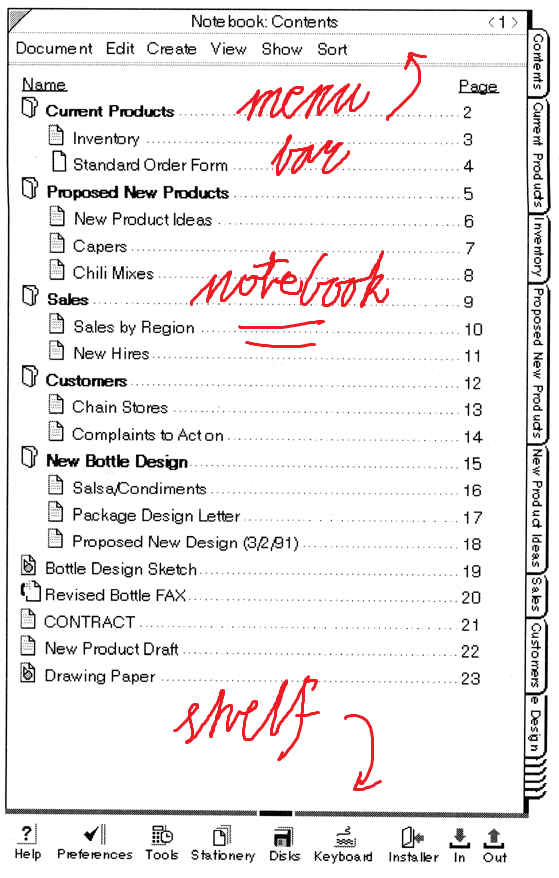
\includegraphics[width=0.5\linewidth]{penpoint-interface-1.png}
    \caption{PenPoint OS: Notebook User Interface}
    \label{fig:notebook-user-interface1}
\end{figure}

The notebook consists of a table of contents in the middle, tabs on the right
that simulate tabs such as those in a three-ring binder, and an optional ``cork
margin'' at the bottom \ref{fig:notebook-user-interface2}. The table of contents
is where all user data is organised. Each document is presented as a page in
the summary. Pages might also be grouped into sections, and sections can be
nested as well, which allows creation of hierarchies similar to directories and
files. Each document is also analogous to a program, this is a part of the EDA.
The tabs allow to jump instantly to a page or a section in the notebook.
PenPoint also allows programs to use tabs for their internal navigation.

\begin{figure}[!h]
    \centering 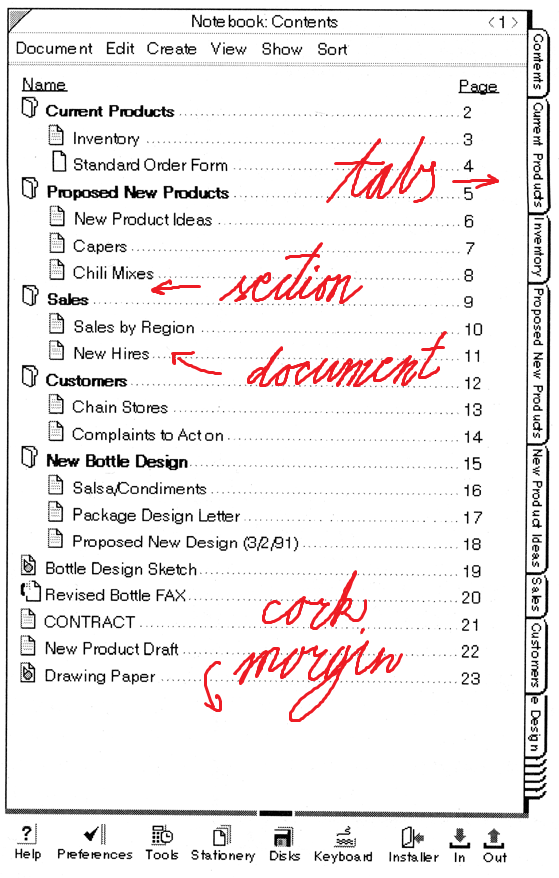
\includegraphics[width=0.5\linewidth]{penpoint-interface-2.png}
    \caption{PenPoint OS: Notebook User Interface}
    \label{fig:notebook-user-interface2}
\end{figure}

The ``cork margin'' is a place attached to the bottom of any document frame that
can contain any PenPoint object \ref{fig:cork-margin}. It is named that because
you can ``pin'' things there as on a cork board. It is turned off by default.

\begin{figure}[!h]
    \centering 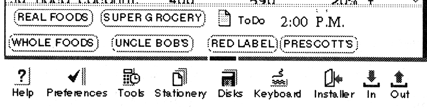
\includegraphics[width=0.5\linewidth]{cork-margin.png}
    \caption{PenPoint OS: Cork Margin}
    \label{fig:cork-margin}
\end{figure}

In Embedded Document Architecture every file is also equivalent to an instance
of a program. Clicking a page opens up the file in the associated application,
there is no distinction between them. There is no notion of saving or loading
\cite{startupadv}, everything is always ready to go. This is what a document is
in PenPoint \cite{carr1991} \cite{brown1992}. But a more important and
impressive aspect of EDA is the ``embedded'' part. In PenPoint every document
has the ability to embed every other document, and this nesting can go as far
as the hardware is capable of. This goes from simple stuff like writing pads
\ref{fig:embedded-document-architecture} - areas that are used for text input,
that could be of different sizes, floating or docked, with input fields
separated into cells or continuous, or signature pads - to things like
pluggable spellcheck or even to embedding a whole drawing program inside of
a presentation, for example.  EDA also allows to copy any and all objects from
one document to another without any loss of quality or information
\cite{carr1991} \cite{brown1993}. In PenPoint the gestures are global and
present all throughout; however it is up to the ``surface'' the gesture was issued
on to decide what it means. Inside a writing pad it is interpreted as a letter,
whereas in a drawing document it could be either interpreted as a shape or an
editing gesture: delete, select, etc. The embedding was not only a useful
functionality, but it also created a greater code reuse and thus lowered the
hardware requirements.

\begin{figure}[!h]
    \centering 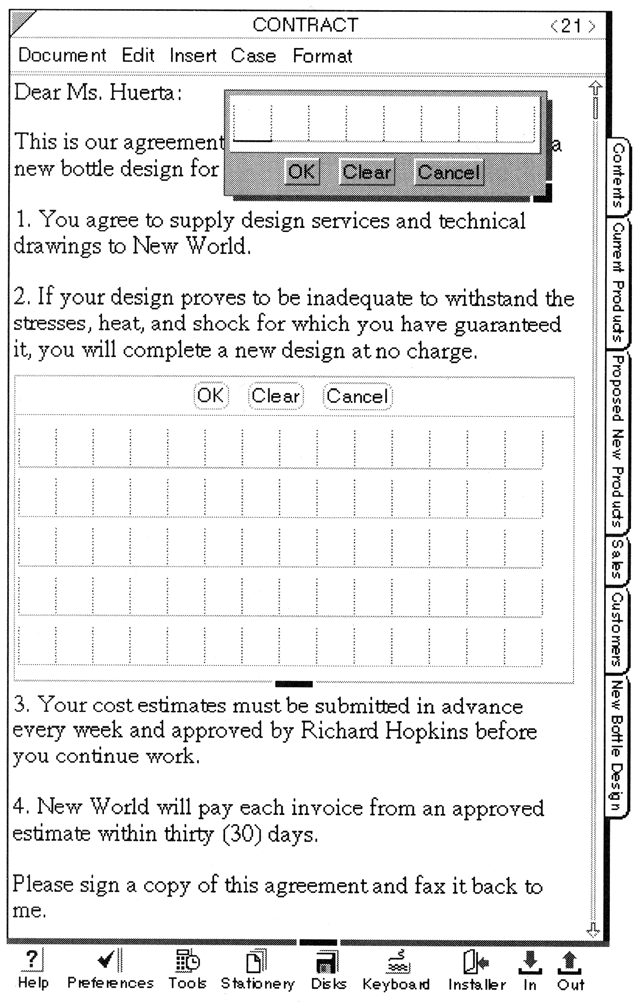
\includegraphics[width=0.5\linewidth]{penpoint-interface-3.png}
    \caption{PenPoint OS: Embedded Document Architecture - writing pads}
    \label{fig:embedded-document-architecture}
\end{figure}

The third main idea is the focus on connectivity. One of the goals of PenPoint
was to be as compatible with different communication protocols as possible.
This meant internet and email but also printers and faxes, it also included not
having to restart the computer in order to connect to a new network, which was
not always the case with other devices at the time. Being able to receive fax
on a PenPoint device meant that it was possible to add freehand notes and
drawings to the received image and resend it without any loss of quality, and
without having to print it and scan it \cite{godemo1991}. The focus on
connectivity also manifested itself in the global address book and an unified
inbox and outbox present in PenPoint. One innovative feature of the PenPoint
outbox was delayed I/O. The delayed I/O was a functionality whereby it was
possible to write and ``send'' an email without a need for internet connection,
with the system scheduling the message to be actually sent when the connection
was present again \cite{carr1991} \cite{brown1993}.

Although I would consider them to be a part of NUI, gestures \ref{fig:gestures}
deserve special attention. What made them so powerful is the fact that
a gesture specifies both the target and the command given - crossing out a word
applies the delete operation on that word, crossing out a shape deletes the
shape. Because of this it was important to provide a lot of gestures and make
them work seamlessly. Gestures and their recognition were implemented on
a system level but it was up to the program to interpret a gesture and act on
it. PenPoint provides about a dozen core gestures that work uniformly across
all the apps with common commands, so a delete or edit gesture would work just
as well on a word, a drawn object or a calendar entry.  Additionally, there are
many more gestures that were application specific.

\begin{figure}[!h]
    \centering 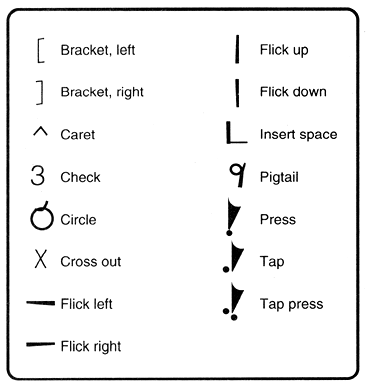
\includegraphics[width=0.5\linewidth]{gestures.png}
    \caption{PenPoint OS: Gestures}
    \label{fig:gestures}
\end{figure}

Nowadays there is lesser interest in a compelling user interface metaphor.
Instead the metaphors encompass only a small portion of the whole, and the
designs are becoming more self-referential - they rely on the familiarity with
the previous versions or similar environments rather than something universal.
Although a smartphone with a touch screen is probably the most popular device,
the use of gestures is minimal, other than simple swipes to go back and switch
between applications, and the extremely powerful notion of target and command
that a gesture provides is non-existent. Some applications, especially centred
around phones employ the PenPoint idea of a document where the data and the
program go hand in hand, and there is no loading or saving. And some even try
to do the embedding part, but the embedding is usually very much limited
compared to what was possible in PenPoint, and requires additional resources
because it is not supported on the system level. Features like unified inbox
and delayed I/O are also missing from modern devices. Some programs have
similar concepts but without inbuilt system support these functionalities just
can not reach full potential, and even though a reliable connection is almost
always available, there is still 1\% of situations where delayed I/O would be
incredibly useful.

\subsection{PenPoint OS: Too great a vision}

PenPoint OS failed. It did not become successful and today is mostly forgotten,
even though a great deal of its original features are still used in today's
operating systems, and many are still missing or unmatched in capability to the
ones PenPoint offered. A large set of gestures that worked system-wide and
``press and hold'' for any selection, a dynamic layout toolkit which allowed
applications to automatically rescale for portrait or landscape orientation,
a global pluggable address book and support for as many connection standards as
possible, as well as automatic scheduling of operations that required
connection for when that connection would be established, like sending or
receiving emails, a document architecture where each document was an instance
of a program and each document could nest another document. All of these were
either innovated or advanced by PenPoint. PenPoint OS was extremely well
designed with the pen-centricity and mobility in mind, and it was coherent in
that design. The notebook interface metaphor was present throughout the whole
user interface.

Despite all of this PenPoint OS did not gain adoption. The biggest and most
obvious problem was the hardware available at the time. Even though the
developers employed many clever solutions and tricks that allowed PenPoint to
operate on a variety of different computers and scale with the available
resources, the problem that could not be overcome was that the technology
required just was not there back then - the screens were dim and low resolution,
the latency was high and the handwriting recognition was not up to par. Even
now, after over 30 years of rapid hardware evolution and incredible leaps in
technology later with resolutions so high and latencies so low that pixels and
delays are virtually imperceivable, writing on a digital device feels off to
many people. In spite of countless advantages offered by the digital, the
feeling of pen and paper still feels superior.

\subsection{Evolution of graphical interfaces: looking back to move forward}

The advancements in graphical user interfaces do not seem to be able to keep up
with the ever growing complexities of the software. In fact, apart from
aesthetic stylistic changes, there is not a lot of change at all, and in some
aspects it could be argued that GUIs are regressing. The proceeding unification
of interfaces across the web and desktop applications and computers, tablets,
and smartphones makes it easier for developers to create new software and for
the users to become familiar with it, but makes it impossible to use any of the
domains to the fullest. In almost all cases a non-graphical or mix of graphical
representation and non-graphical input provides greater possible speed. That is
why many professionals still use text based interfaces or opt for workflows
relying heavily on keyboard shortcuts. The advantages of graphical user
interfaces used to be ease of use and discoverability. This, however, slowly
begins to be less and less the case - with applications being more and more
advanced and providing more and more features, the cascading menus become more
and more crammed and overloaded, and thus less welcoming. The use of gestures
had a little bit of a resurgence with the adoption of bigger touchpads and
touch sensitive screens in laptops. These unfortunately often work only at
a system level or are not uniformly supported across applications. The most
widely used alternative form of input are voice commands. Voice control
unfortunately is only useful at times when any other method is not possible or
not easily accessible like operating navigation while driving or smart home
without moving from the couch. It is not adequate for use in the office or in
loud public places.

As it often happens in engineering, good ideas, sometimes brilliant ideas are
discarded and forgotten because they are held back by the technology available.
And sometimes an entire approach to a problem is rejected as wrong. But then
the knowledge and state of the art changes and these ideas and approaches have
to be discovered all over again. That is why knowing past solutions and looking
there for current and future solutions can yield great results. Those who do
not know the history are bound not to remember that one thing that someone else
did that one time and it did not work but might work now.


\clearpage % Rozdziały zaczynamy od nowej strony.

\section{Goal}

The aim of this work is to achieve a way of running PenPoint OS on a modern
hardware with performance that would make possible to use in a comfortable
manner.  It should be possible to use a mouse, a graphics tablet or a touch
screen for pointing.  This work could be then further used for purposes of
digital preservation of the PenPoint Operating System.

%\subsection{Prior Art}

\clearpage

\section{Prior Art}

% - not popular, not much activity, forgotten system
% - strategies: QEMU, DOSBox, VirtualBox
% - difficult to do - special hardware, documentation lost (of hardware)
% - only ___ Schubiger
% - remaking of the Schubiger solution

% - forgotten system
% - no interest
% - only schubiger
% -
% - difficulty with PPOS
% - multiple versions
% - hardware
% - lost documentation
% -
% - strategies
% - rewrite
% - compatibility layer (wine)
% - emulator
% - VB, QEMU
% -
% - schubiger solution
% -
% - remaking of schubiger solution

Unfortunately there is not much interest in the revival oft the PenPoint
operating system.  Sadly, it is pretty much a forgotten system.  The only other
effort I came across that was dedicated to making PenPoint accessible and
usable again was the project of professor Simon Schubiger.

What makes this task difficult is how many different version of PenPoint there
were.  PenPoint OS was released for a variety of computers, and most of them
had some special, rather unique components.  To make it worse, a lot of
information about that specific hardware is probably lost to time; what is more,
so are the copies of PenPoint installation media for many of these devices.

There are many possible strategies when it comes to making software accessible
for a platform that this software was not intended for originally.  Sometimes
it is possible to modify parts of the source code to port it or even rewrite
the whole thing from scratch if preferable and necessary.  This is almost
always not possible and not feasible.  When the source and destination
platforms are similar enough, some sort of compatibility layer can be used.
Wine works this way to allow running Windows applications on Unix-like systems.
However the most popular and versatile tool for this task is an emulator.
There is a great deal of variety in the available emulators, many of them aim
to solve different, sometimes contradictory problems.  The two most popular
open-source and libre emulators are QEMU and VirtualBox.  The goal of the
former is performance, the goal of the latter is compatibility and best
possible experience out of the box.

Professor Simon Schubiger chose the JPC emulator.  The JPC emulator is
a relatively simple emulator, especially compared to such programs as QEMU, and
it is written in Java.  These features made it easy to create a runnable proof
of concept implementation that allowed to access PenPoint OS.  Unfortunately, it
was not good enough for actual usage.  It was, however, a starting point.  In
the following sections I will describe in greater detail what JPC is, the
modifications created by professor Simon Schubiger, and the attempt to recreate
the running PenPoint solution and port it to QEMU.

\clearpage % Rozdziały zaczynamy od nowej strony.

\section{Modifying QEMU source to run PenPoint OS}

In this first part I will describe what the JPC emulator is and show the
patches created by prof. Simon Schubiger that allow it to run PenPoint OS, as
well as explain why it is not suitable for our goal. Then I will present the
architecture of the QEMU emulator and the reasons it was chosen as the
appropriate solution, and finally I will show how I tried to port the changes
created by prof. Schubiger to the QEMU source.

\subsection{PenPoint for NCR 3125 tablet}

The creators of PenPoint knew that wide adoption would be hard if the barrier
to entry were high. That is why many different versions of PenPoint were created
that could be installed and run on a variety of hardware \cite{carr1991}.

One of those devices was a NCR 3125 \ref{fig:ncr3125} tablet. Although many
tablet-like devices already existed at this point, the System 3125 was the
second pen based computer, the first computer with an external pen
\cite{hohl2014}, and the first pen based computer powerful enough to run
desktop programs like spreadsheet and graphing software \cite{mcdonald2011}.
All of this came at a price - it was one of the most expensive computers
released at the time \cite{hohl2014}. Apart from PenPoint, the NCR 3125 also run
MS-DOS with NCR PenOS - proprietary NCR software that allowed for text input
using the stylus, as well as Windows for Pen Computing and GRiD PenRight
\cite{stengel}.

\begin{figure}[!h]
    \centering
    \begin{subfigure}[b]{0.55\linewidth}
        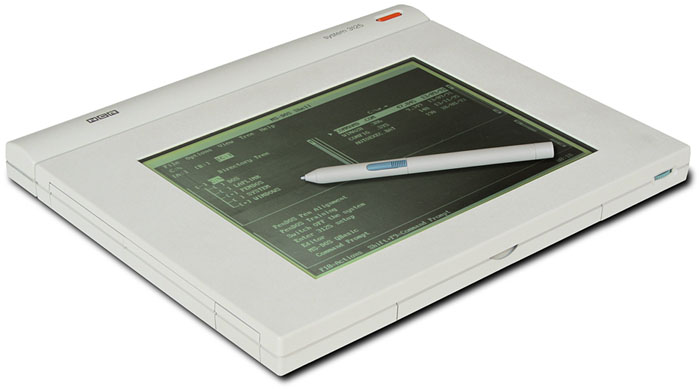
\includegraphics[width=\linewidth]{ncr3125-1.jpg}
        %\caption{NCR 3125}
        %\label{fig:ncr3125-2}
    \end{subfigure}
    \hfill
    \begin{subfigure}[b]{0.35\linewidth}
        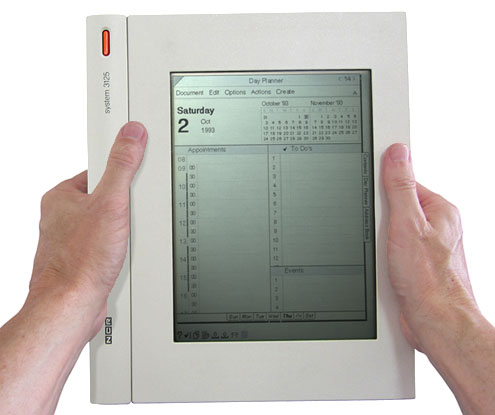
\includegraphics[width=\linewidth]{ncr3125-2.jpg}
        %\caption{NCR 3125}
        %\label{fig:ncr3125-1}
    \end{subfigure}
    \caption{NCR 3125}
    \label{fig:ncr3125}
\end{figure}

The NCR System 3125 was one of the flagship PenPoint computers and its
hardware, apart from the WACOM digitizer, was rather standard x86, thus making
the PenPoint OS version for it an appropriate choice for emulation.

\subsection{The JPC emulator}

JPC was created by the University of Oxford's Particle Physics Subdepartment.
Although its github page claims it is fast, it was not its main concern. The
advertised features are the flexibility, security, and it being cross-platform,
given that it is written in 100\% JAVA programming language. These come however
at a cost. The JAVA environment makes it so that JPC can run virtually on any
hardware that JVM is available for, and the memory safety provided by the JVM,
as well as sandboxing provide great security. This, however, comes at a cost, it
will most certainly be much slower than a highly optimised emulator written in
a systems programming language like C or C++. In fact, the JPC emulator was too
slow to run PenPoint OS at a speed that would be comfortable for use - the
video showing the operation of PenPoint on JPC on professor's Schubiger channel
had to be sped up to look normal \cite{schubiger2015}.

In the following sections I will show how the JPC emulator works and how it is
designed. Then I will describe the modifications to the source code created by
prof. Simon Schubiger that allow it to run PenPoint OS.

\subsubsection{Architecture of JPC}

The architecture of the JPC emulator is somewhat simple, at least when it comes
to such complex software as a virtual machine. There is a class PC that models
the machine being emulated. It stores all the components and manages them. It
uses a different class implementing the PCConfig interface to provide
configuration. The main function processes the input arguments and, based on
them, initialises object of the \emph{PC} class. Input arguments control such things
as setting which files are used as harddrives or floppies, as well as choosing
the boot device out of them.

\begin{codeblock}
    \lstinputlisting[
        caption={PC.java},
        language=Java,
        linerange={1109-1110,1156-1170},
    ]{PC.java}
\end{codeblock}

% Fragment kodu źródłowego programu
% \addmargin pozwala na wcięcie kodu od lewej (tu: 8mm).
% Wcięcie służy do tego, aby numery linii nie wystawały poza lewy margines.
% Druga liczba oznacza wcięcie od prawej.
%\begin{minipage}{\linewidth}
%    \begin{addmargin}[8mm]{0mm}
%        \begin{lstlisting}[
%            language=Java,
%            numbers=left,
%            firstnumber=1,
%            %    caption={\emph{Hello world} w HTML},
%            aboveskip=10pt
%            ]
%public static void main(String[] args) {
%    try {
%
%        // ...
%
%        PC pc = new PC(new VirtualClock(), args, Calendar.getInstance());
%        pc.start();
%        try {
%            while (true) {
%                pc.execute();
%            }
%        } finally {
%            pc.stop();
%            LOGGING.log(Level.INFO, "PC Stopped");
%            pc.getProcessor().printState();
%        }
%    } catch (IOException e) {
%        System.err.println("IOError starting PC");
%    }
%}
%        \end{lstlisting}
%    \end{addmargin}
%\end{minipage}

% https://tex.stackexchange.com/a/286097
The responsibility of the configuration provider class is to add all the
necessary objects representing hardware components to the PC class object. It
does so in four steps using methods \emph{configureMotherboard},
\emph{configurePeripherals}, \emph{configurePCI}, and \emph{configureBIOS}. The
meaning of these functions is rather superficial, as all of them add instances
of classes implementing \emph{HardwareComponent} interface to the list of all
components managed by the PC class object.


\begin{codeblock}
    \lstinputlisting[
        caption={PC.java},
        language=Java,
        linerange={122-122,141-149},
    ]{PC.java}
\end{codeblock}

%\begin{minipage}{\linewidth}
%    \begin{addmargin}[8mm]{0mm}
%        \begin{lstlisting}[
%            language=Java,
%            numbers=left,
%            firstnumber=1,
%            %    caption={\emph{Hello world} w HTML},
%            aboveskip=10pt
%            ]
%public PC(Clock clock, DriveSet drives, int ramSize, Calendar startTime,
%PCConfig config) throws IOException {
%
%    // ...
%
%    config.configureMotherboard(this, startTime);
%    config.configurePeripherals(this);
%    config.configurePCI(this);
%    config.configureBIOS(this);
%
%    if (!configure()) {
%        throw new IllegalStateException("PC Configuration failed");
%    }
%}
%        \end{lstlisting}
%    \end{addmargin}
%\end{minipage}


The next step is the setting up of all of the managed devices. In the
configuration phase all components are made aware of all the other components,
so that they can initialise themselves and establish relations. Here all
devices must connect to the buses, displays and ports as they require. This is
done by repeatedly calling each of the components' method \emph{acceptComponent} to
accept every other component until all components report being fully
initialised.

\begin{codeblock}
    \lstinputlisting[
        caption={PC.java},
        language=Java,
        linerange={447-466},
    ]{PC.java}
\end{codeblock}
            
%\begin{minipage}{\linewidth}
%    \begin{addmargin}[8mm]{0mm}
%        \begin{lstlisting}[
%            language=Java,
%            numbers=left,
%            firstnumber=1,
%            %    caption={\emph{Hello world} w HTML},
%            aboveskip=10pt
%            ]
%private boolean configure() {
%    boolean fullyInitialised;
%    int count = 0;
%    do {
%        fullyInitialised = true;
%        for (HardwareComponent outer : parts) {
%            if (outer.initialised()) {
%                continue;
%            }
%            for (HardwareComponent inner : parts) {
%                outer.acceptComponent(inner);
%            }
%            fullyInitialised &= outer.initialised();
%            if(!fullyInitialised && count > 90)
%            LOGGING.log(Level.WARNING, outer + " not initialized, retry");
%        }
%        count++;
%    } while ((fullyInitialised == false) && (count < 100));
%
%    // ...
%
%        \end{lstlisting}
%    \end{addmargin}
%\end{minipage}

Then also auto-configuration of all PCI devices that is normally done by BIOS
is performed by calling \emph{biosInit} method on all components that are
instances of \emph{PCIBus} class. At this point all the PCI buses are aware of
the PCI connected devices, as they were supposed to register themselves in their
\emph{acceptComponent}.

\begin{codeblock}
    \lstinputlisting[
        caption={PC.java},
        language=Java,
        linerange={482-489},
    ]{PC.java}
\end{codeblock}

%\begin{minipage}{\linewidth}
%    \begin{addmargin}[8mm]{0mm}
%        \begin{lstlisting}[
%            language=Java,
%            numbers=left,
%            firstnumber=21,
%            %    caption={\emph{Hello world} w HTML},
%            aboveskip=10pt
%            ]
%    for (HardwareComponent hwc : parts) {
%        if (hwc instanceof PCIBus) {
%            ((PCIBus) hwc).biosInit();
%        }
%    }
%    return true;
%}
%        \end{lstlisting}
%    \end{addmargin}
%\end{minipage}

Inside \emph{biosInit} the bus initialises devices based on their device class,
vendor, and device IDs, as well as based on whether it uses an I/O port or memory
mapped port I/O regions. The device class specifies what type of device it is.
This is checked so that some special initialisation can be done if the device
is a network controller. Vendor ID and Device ID are checked additionally if
needed - these designate the exact brand and model of the device. The
difference between port mapped and memory mapped I/O regions is that the memory
mapped ones use the same bus as memory and use the same set of instructions to
store and load, whilst the port mapped use special port bus and adequately use
different instructions for reading and writing than normal memory.

Finally the \emph{main} function calls in an infinite loop the \emph{execute}
method of the \emph{PC} object that executes instructions in processor's
current mode by calling functions of objects representing both processor and
address spaces.

\subsubsection{Implementation of JPC modifications for running PenPoint OS}

In this section I will explain what changes have been made by professor
Schubiger in order to make PenPoint OS work in the JPC emulator, as well as how
they work. First I will offer an overview of what has been changed and then
I will describe in detail three classes representing components of the NCR
System 3125 that were necessary for the purposes of its emulation.

To configure the object of the \emph{PC} class that represents the emulated
machine, a class extending \emph{PCConfig} - the \emph{NCR3125} class -  was
created. It also provides the entry point - the \emph{main} function - to this
modified version of JPC. It is pretty much the same as the original, but
slimmed down by removing all of the argument parsing. The \emph{PC} class
object is also initialised using this new \emph{NCR3125} class. The difference
lies in the components that are added in the configuration methods, especially
the components that were specially created for the emulation of the NCR 3125.
Two configuration methods from \emph{PCConfig} are overridden in the
\emph{NCR3125}: \emph{configureBIOS} and \emph{configurePeripherals}. The
\emph{configureBIOS} method is the same as the original - it adds the system
BIOS and VGA BIOS, but conditional adding of sound devices is removed. Changes
to \emph{configurePeripherals} are more substantial.

\begin{codeblock}
    \lstinputlisting[
        caption=NCR3125.java,
        language=Java,
        linerange={48-64},
    ]{NCR3125.java}
\end{codeblock}

%\begin{minipage}{\linewidth}
%    \begin{addmargin}[8mm]{0mm}
%        \begin{lstlisting}[
%            language=Java,
%            numbers=left,
%            firstnumber=1,
%            %    caption={\emph{Hello world} w HTML},
%            aboveskip=10pt
%            ]
%protected void configurePeripherals(PC pc) {
%    pc.add(new Intel82360SL());
%    pc.add(new PIIX3IDEInterface());
%    pc.add(new CLGD6410());
%    pc.add(new Port80(PORT80_CODES));
%    pc.add(new SerialPort(0));
%    pc.add(new SerialPort(1));
%    pc.add(new ParallelPort(0));
%    pc.add(new ParallelPort(1));
%    NCRWacom wacom = new NCRWacom();
%    pc.add(wacom);
%    pc.add(pc.keyboard = new Keyboard(wacom));
%    pc.add(new FloppyController());
%    pc.add(new PCSpeaker());
%}
%        \end{lstlisting}
%    \end{addmargin}
%\end{minipage}

Conditionally adding an ethernet device is removed completely. Third and fourth
\emph{SerialPort}'s are replaced by \emph{ParallelPort} one and two. The
\emph{ParallelPort} class added by professor Schubiger allows for 8 bit reads
and writes to three addresses: \emph{PDATA}, \emph{PSTAT} and \emph{PCON}.
Writes to \emph{PDATA} are logged to the console. There is also a component of
class \emph{Port80} added. This object registers itself with the
\emph{IOPortHandler} with the port 0x80 requested. This port is used for
``power-on self test'' (POST) codes. This class simply logs what kind of test is
performed by writing out code value and summary of the code in the 8 bit write
method. Such a facility could certainly prove useful when debugging, especially
when creating representations of computer components. 

Finally there are also added components representing an Intel 82360SL
processor, Cirrus Logic CLGD6410 VGA controller, and a WACOM digitizer. These
will be described in more detail in the following sections.

\subsubsubsection{The WACOM digitizer}

The \emph{NRCWacom} class representing the WACOM digitizer implements three
interfaces: \emph{IODevice}, \emph{IMouseHandler} and \emph{TimerResponsive}.

The \emph{IMouseHandler} interface requires only one method: \emph{mouseEvent},
which is called to update the state of the pointer. It receives the coordinates
of the pointer, as well as the displacement, and also int \emph{buttons} with
bits set corresponding to pressed down buttons. Particularly, if the first bit
is set, this means that the pen is firmly against the digitizer and if the second
or third bit is set, this means that the button on the pen is pressed.

\begin{codeblock}
    \lstinputlisting[
        caption=NCRWacom.java,
        language=Java,
        linerange={233-239},
    ]{NCRWacom.java}
\end{codeblock}

%\begin{minipage}{\linewidth}
%    \begin{addmargin}[8mm]{0mm}
%        \begin{lstlisting}[
%            language=Java,
%            numbers=left,
%            firstnumber=1,
%            %    caption={\emph{Hello world} w HTML},
%            aboveskip=10pt,
%            columns=fixed,
%            ]
%public void mouseEvent(int x, int y, int z, int dx, int dy, int dz, int buttons)
%{
%    Dimension dim = display.getDisplaySize();
%    this.absx = (int) ((0.87f * x / dim.width)  * NCR_NCRMAXX) + 30;
%    this.absy = (int) ((0.94f * y / dim.height) * NCR_NCRMAXY) + 30;
%    this.buttons = buttons;    
%}
%        \end{lstlisting}
%    \end{addmargin}
%\end{minipage}

Implementing \emph{IMouseHandler} allows the \emph{Keyboard} class to use
\emph{NRCWacom} object as a mouse handler.

The \emph{TimerResponsive} interface is implemented so that a \emph{Timer}
object could call a \emph{callback} method specified by the interface. Inside
the \emph{callback} method the \emph{NCRWacom} fills a ``packet'' of 6 bytes
with status of the digitizer, position of the pen and pressed buttons.

\begin{codeblock}
    \lstinputlisting[
        caption=NCRWacom.java,
        language=Java,
        linerange={241-268},
    ]{NCRWacom.java}
\end{codeblock}

%\begin{minipage}{\linewidth}
%    \begin{addmargin}[8mm]{0mm}
%        \begin{lstlisting}[
%            language=Java,
%            numbers=left,
%            firstnumber=1,
%            %    caption={\emph{Hello world} w HTML},
%            aboveskip=10pt
%            ]
%public void callback() {
%    fillPacket();
%
%    if(streammode != 0) {
%        status |= NCR_DATA_READY;
%        timer.setExpiry(clock.getEmulatedNanos() + interval);
%        irqDevice.setIRQ(irq, 1);
%    }
%}
%
%private void fillPacket() {
%    packet[0] = (byte)(NCR_NCRTAB | NCR_NCRREADY);
%    if     (absx < 0) absx = 0;
%    else if(absx > NCR_NCRMAXX) absx = (int) NCR_NCRMAXX;
%    if     (absy < 0) absy = 0;
%    else if(absy > NCR_NCRMAXY) absx = (int) NCR_NCRMAXY;
%
%    packet[1] = (byte)(absx >> 8);
%    packet[2] = (byte)absx;
%    packet[3] = (byte)(absy >> 8);
%    packet[4] = (byte)absy;
%    packet[5] = 0;
%    if((buttons & 0x1) != 0) packet[5] |= NCR_NCRPENZ;
%    if((buttons & 0x6) != 0) packet[5] |= NCR_NCRBUTTON;
%}
%        \end{lstlisting}
%    \end{addmargin}
%\end{minipage}

This ``packet'' is then read by 8 bit I/O reads from the data register.

\begin{codeblock}
    \lstinputlisting[
        caption=NCRWacom.java,
        language=Java,
        linerange={148-171},
    ]{NCRWacom.java}
\end{codeblock}

%\begin{minipage}{\linewidth}
%    \begin{addmargin}[8mm]{0mm}
%        \begin{lstlisting}[
%            language=Java,
%            numbers=left,
%            firstnumber=1,
%            %    caption={\emph{Hello world} w HTML},
%            aboveskip=10pt
%            ]
%public int ioPortRead8(int address) {
%    switch(address) {
%        case NCR_DATA_REG:
%        int result = 0;
%        if(echobackptr >= 0) {
%            result = echoback[echobackptr++];
%            if(echobackptr >= echoback.length) {
%                echobackptr = -1;
%            }
%        } else {
%            result = packet[packetptr++];
%            if(packetptr >= packet.length) {
%                packetptr = 0;
%                status &= ~NCR_DATA_READY;
%                irqDevice.setIRQ(irq, 0);
%            }
%        }
%        return result;
%        case NCR_STATUS_REG:
%        return status;
%    }
%    return super.ioPortRead8(address);
%}
%        \end{lstlisting}
%    \end{addmargin}
%\end{minipage}

The \emph{Timer} object is created from the \emph{Clock} object. The
\emph{Clock} object, along with \emph{InterruptController} and
\emph{IDisplayAdapter}, are obtained and set during the component initialisation
stage performed by the \emph{PC} object by calling \emph{acceptComponent}
method. The \emph{IDisplayAdapter} is used to get dimensions of the display in
the \emph{mouseEvent} method, and the \emph{InterruptController} is used to
raise interrupt when the ``packet'' is filled and unset it when the ``packet''
is wholly read. Apart from these objects, an instance of \emph{IOPortHandler} is
used to register \emph{NCRWacom} as capable for I/O using
\emph{registerIOPortCapable}. What this means will be explained in the next
paragraph.

Finally the \emph{IODevice} interface is the most important piece, as it
provides all of the methods used for I/O, and this is where all of the changing
of the state of the device and most of the logic, as well as reporting of the
state will happen.

\begin{codeblock}
    \lstinputlisting[
        caption=IODevice.java,
        language=Java,
        firstline=3,
    ]{IODevice.java}
\end{codeblock}

%\begin{minipage}{\linewidth}
%    \begin{addmargin}[8mm]{0mm}
%        \begin{lstlisting}[
%            language=Java,
%            numbers=left,
%            firstnumber=1,
%            %    caption={\emph{Hello world} w HTML},
%            aboveskip=10pt
%            ]
%public interface IODevice {
%
%    public void ioPortWrite8(int address, int data);
%
%    public void ioPortWrite16(int address, int data);
%
%    public void ioPortWrite32(int address, int data);
%
%    public int ioPortRead8(int address);
%
%    public int ioPortRead16(int address);
%
%    public int ioPortRead32(int address);
%
%    public int[] ioPortsRequested();
%}
%        \end{lstlisting}
%    \end{addmargin}
%\end{minipage}

The \emph{NCRWacom} overrides three methods used for I/O. To let the
\emph{IOPortHandler} object know what ports are needed, \emph{ioPortsRequested}
method is used. Apart from that, methods for 8 bit read and write are provided:
\emph{ioPortRead8} and \emph{ioPortWrite8}. The \emph{ioPortRead8} allows
reading from two addresses: the status register returns if the device is ready
for command (always set), and if data - the ``packet'' is ready; the data
register contains either a set of predefined values if it was not previously
read or if \emph{NCR\_ECHOBACK} command was issued, or else it contains
consecutive bytes of the ``packet''. Otherwise implementation of
\emph{ioPortRead8} from the superclass - \emph{AbstractHardwareComponent} is
called, which just prints to console.

The \emph{ioPortWrite8} writes to either data register which is a noop or to
command register, otherwise again the write is delegated to the superclass
which does a print to console.

\begin{codeblock}
    \lstinputlisting[
        caption={},
        language=Java,
        linerange={99-104},
    ]{NCRWacom.java}
    \dots
    \lstinputlisting[
        caption=NCRWacom.java,
        language=Java,
        linerange={142-146},
    ]{NCRWacom.java}
\end{codeblock}

%\begin{minipage}{\linewidth}
%    \begin{addmargin}[8mm]{0mm}
%        \begin{lstlisting}[
%            language=Java,
%            numbers=left,
%            firstnumber=1,
%            %    caption={\emph{Hello world} w HTML},
%            aboveskip=10pt
%            ]
%public void ioPortWrite8(int address, int data) {
%    switch(address) {
%    case NCR_DATA_REG:
%        break;
%    case NCR_COMMAND_REG:
%        // ...
%        \end{lstlisting}
%        \begin{lstlisting}[
%            language=Java,
%            numbers=left,
%            firstnumber=42,
%            %    caption={\emph{Hello world} w HTML},
%            aboveskip=10pt
%            ]
%        break;
%    default:
%        super.ioPortWrite8(address, data);
%    }
%}
%        \end{lstlisting}
%    \end{addmargin}
%\end{minipage}

There are a few possible commands that can be written to the command register.
Commands \emph{NCR\_STREAMSTOP} and \emph{{NCR\_RESET}} turn off stream mode.
Stream mode makes it so that the callback invoked by the \emph{Timer} does not
set the next time it is called and does not raise the interrupt.

\begin{codeblock}
    \lstinputlisting[
        caption=NCRWacom.java,
        language=Java,
        linerange={104-111},
    ]{NCRWacom.java}
\end{codeblock}

%\begin{minipage}{\linewidth}
%    \begin{addmargin}[8mm]{0mm}
%        \begin{lstlisting}[
%            language=Java,
%            numbers=left,
%            firstnumber=6,
%            %    caption={\emph{Hello world} w HTML},
%            aboveskip=10pt
%            ]
%    case NCR_COMMAND_REG:
%        switch(data) {
%        case NCR_STREAMSTOP:
%            streammode = 0;
%            break;
%        case NCR_RESET:
%            streammode = 0;
%            break;
%
%        \end{lstlisting}
%    \end{addmargin}
%\end{minipage}

The \emph{NCR\_ECHOBACK} command makes it so the next \emph{ioPortRead}s from
the data register will return values from the predefined ``echo''.

\begin{codeblock}
    \lstinputlisting[
        caption=NCRWacom.java,
        language=Java,
        linerange={112-114},
    ]{NCRWacom.java}
\end{codeblock}

The \emph{NCR\_REQUEST} updates the ``packet'' and sets the data ready bit in
status.

\begin{codeblock}
    \lstinputlisting[
        caption=NCRWacom.java,
        language=Java,
        linerange={115-119},
    ]{NCRWacom.java}
\end{codeblock}

There are also 7 \emph{NCR\_STREAM*} commands that turn on the stream mode and
change interval at which the \emph{Timer} callbacks are set to occur.

\begin{codeblock}
    \lstinputlisting[
        caption=NCRWacom.java,
        language=Java,
        linerange={120-138},
    ]{NCRWacom.java}
\end{codeblock}

\subsubsubsection{The Intel 82360 SL processor}

The interesting thing about the \emph{Intel82360SL} class is that it does not
implement all of the functionality of a processor. In fact it is very simple
and short - all of its logic is contained in 8 bit and 16 bit I/O port read and
write functions. Instead, it is added as a component in addition to the default
\emph{Processor} class used by \emph{PC} class.

The 8 bit write function - \emph{ioPortWrite8} - if called with a write to
address \emph{CFGSTAT} with value of 0 increases value of \emph{unlock} by 1.
This value of \emph{lock} guards writes to several other addresses. It holds
whether configuration space was unlocked and whether the selected unit is
enabled. 

\begin{codeblock}
    \lstinputlisting[
        caption={},
        language=Java,
        linerange={171-173},
    ]{Intel82360SL.java}
    \dots
    \lstinputlisting[
        caption={},
        language=Java,
        linerange={184-187},
    ]{Intel82360SL.java}
    \dots
    \lstinputlisting[
        caption=Intel82360SL.java,
        language=Java,
        linerange={198-199},
    ]{Intel82360SL.java}
\end{codeblock}

Then a 8 bit write to \emph{CPUPWRMODE} when \emph{unlock} is equal to 1 -  so
when configuration space is unlocked - with a value of ``0x80'', that is with all
but most significant bit set, increases value of \emph{unlock} again, and with
that enables selected unit. When the \emph{unlock} value is greater than 2 the
written value is stored in \emph{cpupwrmode}.

\begin{codeblock}
    \lstinputlisting[
        caption=Intel82360SL.java,
        language=Java,
        linerange={174-179},
    ]{Intel82360SL.java}
\end{codeblock}

Similarly, when configuration space is both unlocked and selected unit is
enabled 8 bit writes to \emph{CFGINDEX} store the value written to \emph{idx},
which is later used in the case of 8 bit write to \emph{CFGDATA} which stores write
data into \emph{regs} under previously selected \emph{idx}.

\begin{codeblock}
    \lstinputlisting[
        caption=Intel82360SL.java,
        language=Java,
        linerange={180-183,188-191},
    ]{Intel82360SL.java}
\end{codeblock}

In the default case, the write is delegated to the 16 bit version of the
function by converting the address to 16 bit version through making the address
even by zeroing the lowest bit, performing a 16 bit read from the address to
obtain the other 8 bits, and performing 16 bit write with combined data of the
original write with the value of the other byte. This results in calling the
superclass counterpart of this method, which simply performs printing to
console, since the only address handled by the 16 bit write method is
\emph{CPUPWRMODE}, which is also covered by the 8 bit version.

The 8 bit read function allows to obtain value of \emph{cfgtstat} by reading
from address \emph{CFGSTAT}. This variable is never used nor initialised so it
seems to be a mistake. Reading from address \emph{CFGDATA} bears value
stored in \emph{regs} at index \emph{idx}. Four addresses 0xFFF9, 0xFFFB,
0xFFFD, and 0xFFFF always contain 0. For all other addresses the read is
delegated to the 16 bit version of the function with aligning the address to 16
bits and masking and shifting the result to convert it back to 8 bits.

\begin{codeblock}
    \lstinputlisting[
        caption=Intel82360SL.java,
        language=Java,
        linerange={201-217},
    ]{Intel82360SL.java}
\end{codeblock}

The \emph{ioPortWrite16} method allows for writing to \emph{CPUPWRMODE}
address. Otherwise it reverts to using the superclass implementation, which just
logs the write. Analogically to the 8 bit version it increases the \emph{unlock}
and updates the value of \emph{cpupwrmode} with data written, but it adds to
\emph{unlock} when its value is equal to 2 instead of 1 like the
\emph{ioPortWrite8} does.

The function \emph{ioPortRead16} allows for reads from \emph{PPCONFIG} address
or otherwise prints out information about the read by referring to the same
method in the base class.

\begin{codeblock}
    \lstinputlisting[
        caption=Intel82360SL.java,
        language=Java,
        linerange={149-169},
    ]{Intel82360SL.java}
\end{codeblock}

\subsubsubsection{The Cirrus Logic CLGD6410 VGA controller}

The implementation file for the CLGD6410 VGA controller is rather big,
especially in comparison to the other source modifications provided by
professor Schubiger, spanning just under 3000 lines of code. But it turns out
that a great deal of it is the same as the code for the originally provided VGA
card with minor modifications.

The \emph{CLGD6410} class is pretty much a copy of the \emph{VGACard} class
with additional functionality provided by the class \emph{DefaultVGACard}
included as well. The \emph{DefaultVGACard} normally extends the \emph{VGACard}
class with some utility functions, like getting display dimensions, saving
screenshots or adding monitors. The object of that class is then normally used
as one of the components of a PC. Apart from that, all of the PCI and interrupt
request code is removed, VRAM size is changed, and new addresses for I/O are
added, as well as a bunch of requested I/O ports are used in addition to the
ones in the default implementation. The VGA RAM size is changed from 16M to
256K. Finally, new addresses are added for graphics, sequencer, attribute,
and crt registers to write, as well as new possible values that could be
written.

\subsubsection{Building and running JPC with the patch}

Unfortunately I failed to build and run PenPoint OS with this modified version
myself. The original source code is really old, and targets an outdated Java
version, that my installation would refuse to compile. But even after changing
the target version, fixing some hardcoded paths that were used for resources,
and updating some parts of the code to adhere to the newer version of Java the
program crashed. Despite this I still planned to port these changes to the QEMU
emulator by reading and understanding the logic and intent behind the changes
in the patch.

\subsection{The QEMU hypervisor}

The QEMU emulator is a much more complex piece of software than the JPC
emulator. It has multiple target host and guest architectures - that is, it is
possible for QEMU to run on many diverse types of machines, as well as it is
possible to emulate different computer types. QEMU also offers utility tools
used for emulation purposes, such as creation of disk images, as well as provides
programs both for system emulation and for user emulation - meaning an emulator
for a whole system or or an emulator for a single executable that was compiled
for a different architecture. What is more, QEMU is not only an emulator but it
is actually a hypervisor. In this case, this means that the emulation is not
necessarily done in software only but is also ``hardware accelerated'' in some
way. QEMU has the ability to run guest instructions directly on host hardware
with tiny or negligible overhead.  This can be achieved by using special host
instructions meant for virtualization, and trapping signals. QEMU is also
written in the C programming language, which by its nature is fast, and it also
allows for careful optimization by hand, whether by using handwritten assembly or
by using compiler intrinsics. What is more, QEMU is a free libre open source
software that is actively developed by the community and many big firms are
interested in its improvement. All of that makes QEMU's performance unbeatable,
but also makes for a plethora of other problems and complications.

Being free and open source software under the GPL2 licence, written in C and
with a thriving community makes it great for contributions. Although many open
source projects neglect creating and maintaining documentation, and in case of
projects that often require expert knowledge like that one such behaviour has
a byproduct of filtering out people that would not be adequately equipped to
work on them, QEMU has a rather good documentation even if sometimes lacking or
outdated, at least in comparison to others similarly specialised projects. This,
combined with the immense performance that QEMU offers, makes it suitable for
building modifications that would make it possible to run PenPoint OS on modern
hardware with necessary speed for comfortable use.

In the following sections I will explain how QEMU operates, show the process of
creating a new device in the QEMU source tree, and explain how QEMU's build
system works.

\subsubsection{Operation of QEMU}

In order to support many target host and guest architectures, it is necessary to
decouple implementation of one from the other - perform some sort of ``strength
reduction'' - instead of creating a combination of all possible pairs of host
and guest, it is only required to provide a sum by using an universal
intermediate step. This way the host backend only has to translate host
instructions to one special set of instructions and from there guest frontend
only has to convert from one special set of instructions. Doing it this way has
also the added benefit of adding a new host, new guest or modifying
implementation of existing one without having to change anything else. This is
what Tiny Code Generator (TCG) does. As it turns out, this also helps with
performance optimization.

A basic mode of operation for translating opcodes in an intermediate manner
would be to fetch and convert the instruction. Then some sort of code
initialising the execution environment would be performed, the instruction would
be run, and finally a cleanup would occur. In order to increase the speed of
execution, QEMU fetches multiple instructions at a time for translation.  These
portions of instructions are then converted to what is called a Translation
Block (TB). A Translation Block is created when a branch instruction is
encountered or the internal state of the processor that would affect the
execution is changed. That means that TB's have only a single exit point. It is
not possible to jump to the middle of a Translation Block. In such a situation,
a new TB would have to be created. This means that one Translation Block can
have only one entry and one exit point. After a TB is created, it is inserted
into cache. That way, the next time QEMU needs to execute an instruction it can check
if the corresponding Translation Block was already ready, and completely skip
that stage if possible. In order to execute a TB, the execution environment must
be set up. This is the ``prologue''. After the TB finishes, a cleanup must be
performed. This is the ``epilogue''. Because these ``prologues'' and
``epilogues'' can be quite costly performance wise QEMU can chain multiple TBs
together without ``prologues'' and ``epilogues'' in between. QEMU also performs
several optimizations on the Translation Blocks such as dead code elimination
\cite{qemu2022} \cite{vasut2017}.

\subsubsection{Adding a device code to the QEMU source tree}

QEMU uses an object oriented approach for defining new devices, which would be
great, if it wasn't for the fact that QEMU is written in C programming language.
What this means is that all of the inheritance and method overriding must be done
by hand by the programmer. But that is not all. For this to work, all of that has
to be passed around by either opaque void pointers or pointers to the base
class and stringly type-checked at runtime. Unfortunately, there does not really
exist any official documentation for creating new devices apart from a general
QEMU Object Model (QOM) overview, which only describes the process of registering
a new type. The best we can do is to analyse source code of the educational device
that exists in QEMU repository or read through comments of many source header
files located in different places associated with device creation.

In order for the device to be available to QEMU, it has to be registered. The
way to do this is to create an object that describes the type of the relevant device.
It contains the parent class, as well as information on how both the object
representing class of the device and object representing instance of the
device should be instantiated. Inside the class initialization function all of
the additional data needed to create an instance of the class has to be set, as
well as all of the information required by the parent class. The instance setup
function is responsible for initialising the object that represents the state
of the device. Additionally some classes of devices, like PCI devices, have
their own required functions used for initialization, cleanup or other. The
last step to making the newly created device available to QEMU is adding the
source file to the build system, which is rather complicated to say the least,
so that it is compiled and linked with the desired binary.

In the following subsections I will present an extremely simple example device,
and describe a little more complex educational device that exists within QEMU
source code. In a subsequent section I will show how the QEMU build system
works and how to add a device to be compiled.

\subsubsubsection{Simple example device implementation}

The first thing to do when creating a new device in QEMU is to create structs that
will represent the class and the state of an instance of the device. The object
representing the class should hold all of the methods - the virtual  table, as
well as all of the data associated with the class. The instance struct ought to
contain the internal state of the device. As opposed to the instance struct
objects which are created for every device, the class struct is created only
once for every device type. To declare the new object type, a macro
\emph{OBJECT\_DECLARE\_TYPE} is used with the instance struct, class struct,
and the name of the module. This macro provides the standard type casting
functions and registers the instance struct to be used with \emph{g\_autoptr}
so that it is cleaned up properly. The \emph{TYPE\_TEST} string will be used to
specify this device on the QEMU command line, and although not directly
specified, it is used for type checking in the casting functions defined by
\emph{OBJECT\_DECLARE\_TYPE}.

\begin{codeblock}
    \lstinputlisting[
        caption=test-device.c,
        language=C++,
        linerange={8-18},
    ]{test-device.c}
\end{codeblock}

The next step is to define the methods and the device logic. Because this
device does not do anything, only the basic functions for the class and instance
initialization and for instance cleanup are defined.

\begin{codeblock}
    \lstinputlisting[
        caption=test-device.c,
        language=C++,
        linerange={20-30},
    ]{test-device.c}
\end{codeblock}

The last step is to register the newly created device for use. This is done by
creating a variable of type \emph{TypeInfo} that contains all the necessary
information about the type for its instantiation: the sizes and constructors
for the instance and class objects, as well as the base class and name used to
specify this device on command line. A function that will register this type by
passing this variable as argument has to be defined. And finally, using a macro
\emph{type\_init}, this function is added to the list of functions to be run at
startup so that it is called before main.

\begin{codeblock}
    \lstinputlisting[
        caption=test-device.c,
        language=C++,
        linerange={38-53},
    ]{test-device.c}
\end{codeblock}

\subsubsubsection{The QEMU edu device}

The educational device was created for use in the linux kernel course at
Masaryk University. It is a simple PCI device that can respond to reads and
writes, generates interrupts and performs Direct Memory Access (DMA).

Similarly to the example device from the previous section, it defines the
instance struct and uses a macro to generate the casting functions. It does not
define any class struct because it uses \emph{PCIDeviceClass} without any
modifications. For the same reason \emph{DECLARE\_INSTANCE\_CHECKER} macro can
be used - the machinery for \emph{PCIDeviceClass} was already defined. 

\begin{codeblock}
    \lstinputlisting[
        caption={},
        language=C++,
        linerange={47-49},
    ]{edu.c}
    \dots
    \lstinputlisting[
        caption=edu.c,
        language=C++,
        linerange={78-78},
    ]{edu.c}
\end{codeblock}

The \emph{TypeInfo} variable used for registering the type also has field
\emph{interfaces} initialised. It is a list of used interfaces and in this case
it contains only \emph{INTERFACE\_CONVENTIONAL\_PCI\_DEVICE}.

\begin{codeblock}
    \lstinputlisting[
        caption=edu.c,
        language=C++,
        linerange={425-442},
    ]{edu.c}
\end{codeblock}

In the class initialisation function \emph{edu\_class\_init} additional PCI
specific information has to be set: the PCI class, vendor and device IDs, as
well as two PCI methods: \emph{realize} and \emph{exit}. The instance
initialisation function \emph{edu\_instance\_init} simply sets the DMA mask and
marks it as a property that can be changed on the command line.

\begin{codeblock}
    \lstinputlisting[
        caption=edu.c,
        language=C++,
        linerange={402-423},
    ]{edu.c}
\end{codeblock}

The \emph{realize} PCI function is set to \emph{pci\_edu\_realize}. It sets up
the interrupts, a timer with a callback that will be used for DMA, creates
a thread that will be used for calculating a factorial and initialises a mutex
and condition variable that it will use for synchronisation, finally it
initialises a memory region for I/O.

\begin{codeblock}
    \lstinputlisting[
        caption=edu.c,
        language=C++,
        linerange={362-384},
    ]{edu.c}
\end{codeblock}

The \emph{pci\_edu\_uninit} function is used for PCI \emph{exit}. It makes the
computation thread break out of an infinite loop and joins it, destroys the
mutex, conditional variable and timer, and initialises the MSI interrupt.

\begin{codeblock}
    \lstinputlisting[
        caption=edu.c,
        language=C,
        linerange={385-400},
    ]{edu.c}
\end{codeblock}

The memory mapped I/O read function \emph{edu\_mmio\_read} checks first if the
read size is correct or else it returns early.

\begin{codeblock}
    \lstinputlisting[
        caption=edu.c,
        language=C,
        linerange={189-200},
    ]{edu.c}
\end{codeblock}

\noindent
Then depending on the address it allows to read a register containing an identification value,

\begin{codeblock}
    \lstinputlisting[
        caption=edu.c,
        language=C,
        linerange={202-205},
    ]{edu.c}
\end{codeblock}

\noindent
the computed value of factorial,

\begin{codeblock}
    \lstinputlisting[
        caption=edu.c,
        language=C,
        linerange={209-213},
    ]{edu.c}
\end{codeblock}

\noindent
the status register and interrupt request status register,

\begin{codeblock}
    \lstinputlisting[
        caption=edu.c,
        language=C,
        linerange={214-219},
    ]{edu.c}
\end{codeblock}

\noindent
as well as addresses used for DMA, DMA transfer count and DMA command register.

\begin{codeblock}
    \lstinputlisting[
        caption=edu.c,
        language=C,
        linerange={220-232},
    ]{edu.c}
\end{codeblock}

\noindent
It also allows to read a register providing liveness check by storing bit inverse of value written to it.

\begin{codeblock}
    \lstinputlisting[
        caption=edu.c,
        language=C,
        linerange={206-208},
    ]{edu.c}
\end{codeblock}

The \emph{edu\_mmio\_write} function providing memory mapped I/O writes
similarly to the read function checks first whether the write size is correct.

\begin{codeblock}
    \lstinputlisting[
        caption=edu.c,
        language=C,
        linerange={237-248},
    ]{edu.c}
\end{codeblock}

\noindent
Writing to the factorial register sets the value of which factorial should be
computed next under the condition that a computation is not taking place
already.

\begin{codeblock}
    \lstinputlisting[
        caption=edu.c,
        language=C,
        linerange={250-250,254-257,261-266},
    ]{edu.c}
\end{codeblock}

\noindent
The status register allows to control whether an interrupt should be raised
after finishing factorial computation. Then there are two registers with which
interrupt requests can be raised and acknowledged.

\begin{codeblock}
    \lstinputlisting[
        caption=edu.c,
        language=C,
        linerange={267-279},
    ]{edu.c}
\end{codeblock}

\noindent
Finally there are four registers that are used to change DMA settings: the
source and destination addresses, the transfer count and the command.

\begin{codeblock}
    \lstinputlisting[
        caption=edu.c,
        language=C,
        linerange={280-295},
    ]{edu.c}
\end{codeblock}

The thread whose task is to compute the value of a factorial consists of an
infinite loop. Inside the loop it waits until it is either commanded to finish
or a computation of a new value is requested by a MMIO write to the factorial
register.

\begin{codeblock}
    \lstinputlisting[
        caption=edu.c,
        language=C,
        linerange={317-328},
    ]{edu.c}
\end{codeblock}

\noindent
If it is commanded to finish, it breaks out of the infinite loop.

\begin{codeblock}
    \lstinputlisting[
        caption=edu.c,
        language=C,
        linerange={330-333},
    ]{edu.c}
\end{codeblock}

\noindent
Otherwise it reads the requested value to compute factorial of and enters
a computation loop.

\begin{codeblock}
    \lstinputlisting[
        caption=edu.c,
        language=C,
        linerange={335-340},
    ]{edu.c}
\end{codeblock}

\noindent
After that is done, the value in the factorial register is updated. If an
interrupt request was set using the status register to be issued after
computation of factorial was completed this is done now.

\begin{codeblock}
    \lstinputlisting[
        caption=edu.c,
        language=C,
        linerange={347-360},
    ]{edu.c}
\end{codeblock}

There is also support for Direct Memory Access. Whenever a value is written to
the DMA command register, a timer is set to run the \emph{edu\_dma\_timer}
callback after 100 nanoseconds.

\begin{codeblock}
    \lstinputlisting[
        caption={},
        language=C,
        linerange={289-294},
    ]{edu.c}
    \dots
    \lstinputlisting[
        caption={},
        language=C,
        linerange={171-173},
    ]{edu.c}
    \dots
    \lstinputlisting[
        caption=edu.c
        language=C,
        linerange={184-187},
    ]{edu.c}
\end{codeblock}

The \emph{edu\_dma\_timer} function performs either read or write, based on the
contents of the DMA command register from the address set by the DMA source
register to the address set by the DMA destination register. Then an interrupt
request is raised, based again on the value of the DMA command register.

\begin{codeblock}
    \lstinputlisting[
        caption=edu.c,
        language=C,
        linerange={138-169},
    ]{edu.c}
\end{codeblock}

\subsubsection{QEMU build system}

The QEMU build system is extremely convoluted. It probably started as something
that had to support a large number of targets, architectures and configuration
options but was reasonable, but then it grew and after years it became
unrecognisable. The build process is done in three stages, but to the user it
takes two steps. It uses a meta build system, two build systems and a configure
script underneath. The first stage is the configure script. It is a standard
script written in POSIX SH. It is used to determine the local build
characteristics like what kind of tools and libraries are available. The second
stage uses the Meson meta build system. It also determines the local build
characteristics. Meson also processes \emph{Kconfig} and \emph{*.mak} files
that describe the dependencies among various features and subsystems. The
\emph{Kconfig} files use almost the same language as the linux kernel
\emph{Kconfig} files but only so slightly different. The output of the Meson
stage are \emph{build.ninja} files, but the ninja build tool is not used
directly.  Instead, the files are used to synthesise rules for Make. The final
stage and also the second step for the user is to run Make with the rules
created from the ninja file \cite{qemu2022}.

In order to make the simple example device defined before becoming available to QEMU at
runtime it is only necessary to create a new entry in the \emph{Kconfig} file
in the parent directory of where the source file for the device is located. In
this case a simple \emph{default y} states that the configuration option this
entry denotes will always be true.

\begin{codeblock}
    \lstinputlisting[
        caption=Kconfig,
        language=C,
        linerange={50-52},
    ]{Kconfig}
\end{codeblock}

\noindent
We can do it this way because the device does not depend on anything, does not
provide anything, and frankly does not do anything. Had it more complicated
dependency relationships, one would have to use the \emph{Kconfig} to specify
dependencies, reverse dependencies, default and conditionally default values.
The next step is to modify the \emph{meson.build} file to add the new source
file to the appropriate sourceset if the configuration option created in the
\emph{Kconfig} file is set.

\begin{codeblock}
    \lstinputlisting[
        caption=meson.build,
        language=Python,
        linerange={20-20},
    ]{meson.build}
\end{codeblock}

\noindent
Now, after the changes to the \emph{Kconfig} and \emph{meson.build} files, the
newly created device can be specified on the command line. The output shows
that a class is initialised  once but an instance is created twice - for each
device specified \ref{fig:qemu-test-device-output}.

%\begin{figure}[!h]
\begin{figure}[H]
    \centering
    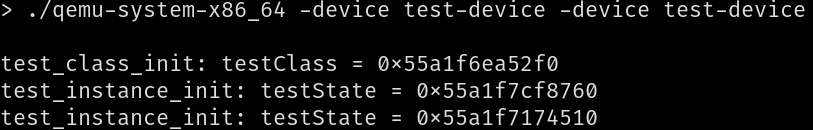
\includegraphics[width=0.9\linewidth]{qemu-test-device-output.png}
    \caption{QEMU test device output}
    \label{fig:qemu-test-device-output}
\end{figure}

\subsection{Conclusion}

%In the end the issues with the modified JPC emulator, the steep learning curve
%for QEMU development and a possibility that debugging something or
%understanding why something does not work could prove simply impossible for me
%or require knowledge that could take years to obtain, especially if the only
%symptom is that the system does not boot, made me abandon QEMU as a platform to
%use. This was also motivated by the fact that a more straightforward solution,
%which will be discussed in the next chapter,  presented itself.

In the end, because of the issues with the modified JPC emulator, and the unnecessary
complexity that fell outside the scope of this work, I decided to consider
a different approach.  In the next chapter a more straightforward and less error
prone solution that uses a developer SDK version of PenPoint OS is discussed.


\clearpage % Rozdziały zaczynamy od nowej strony.

\section{Running PenPointOS on FreeDOS}

In this second part I will explain what FreeDOS and PenPointOS SDK are, and how
to install and run the PenPointOS version intended for developers. Using this
version of PenPoint OS was made possible after one of the commenters on
professor Schubiger original PenPointOS video found the installation media
files hosted on a site dedicated to archiving computer history.

In these following sections I will outline the steps to installing the
PenPointOS version for MS-DOS, and running on QEMU in FreeDOS.

\subsection{PenPoint for DOS}

The creators of PenPointOS knew that users would not choose their operating
system over an established solution, even if it was a better product, had there
not been software written for it. That is why making the barrier to entry for
developers as low as possible, and making them productive as fast as possible
was one of the goals Robert Carr, the architect of PenPoint, outlined as a key
requirement in the book ``The Power of PenPoint'' \cite{carr1991}. The creators
also knew that programmers would not be able or eager to invest in new devices.
That is why the PenPointOS Software Development Kit included a version of
PenPointOS that could be installed on compatible desktop PCs running MS-DOS.

\subsection{What is FreeDOS}

FreeDOS is a free and libre open source operating system licensed under GPL. It
is intended to be fully compatible with MS-DOS environment and is designed to
run well in a virtual machine. FreeDOS has a thriving community. There is
original development of new software, and there programs ported from other
platforms. And everything is well documented.  FreeDOS is easier to use and
much more accessible than the original DOS.  There is even a package manager.
All of those reasons make it a good pick to use for the purposes of running
PenPoint OS.

\subsection{Obtaining the files}

After downloading the files from the bitsavers website the eight floppy disk
images need to be converted in order for them to be used. The .IMD files were
created using a DOS program ImageDisk used to backup floppies. These however
cannot be used with QEMU as the format is not supported. In order for them to
be readable to QEMU these must be converted to .img files. This can be done
using any program that supports converting .IMD files to .img files.

\subsection{Installing PenPointOS on FreeDOS}

After installing FreeDOS in a virtual machine and converting the ImageDisk
files to .img, now it is the time to install PenPoint OS. In order to do so
a floppy device must be added to the VM configuration. Here the file DISK1.img
must be used as source. Inside FreeDOS inserted floppy will be available as A:
drive. To access another drive simply type its name. Finally to run the
installation execute install.exe \ref{fig:fd-main-screen}.

\begin{figure}[H]
    \centering
    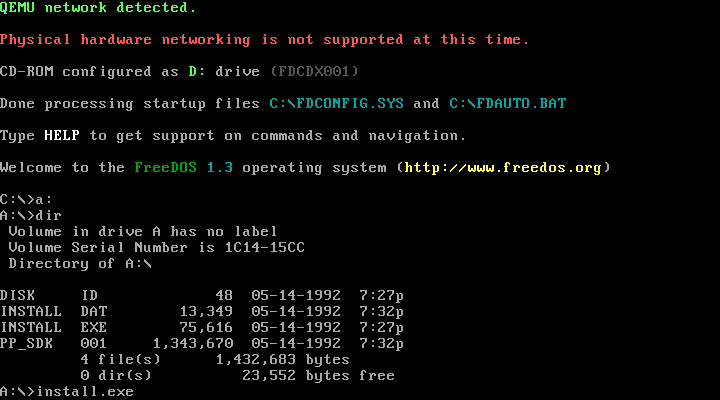
\includegraphics[width=0.9\linewidth]{fd-main-screen.png}
    \caption{FreeDOS: main screen}
    \label{fig:fd-main-screen}
\end{figure}

Then get through the installation wizard by confirming to use the C: drive for
installation and the installation subdirectory \ref{fig:penpoint-installation}.
The default choices are fine.  After installation from the first floppy is
finished the wizard will ask to insert the next disk until the contents of all
eight disks are installed.

\begin{figure}[H]
    \centering
    \begin{subfigure}[b]{0.45\linewidth}
        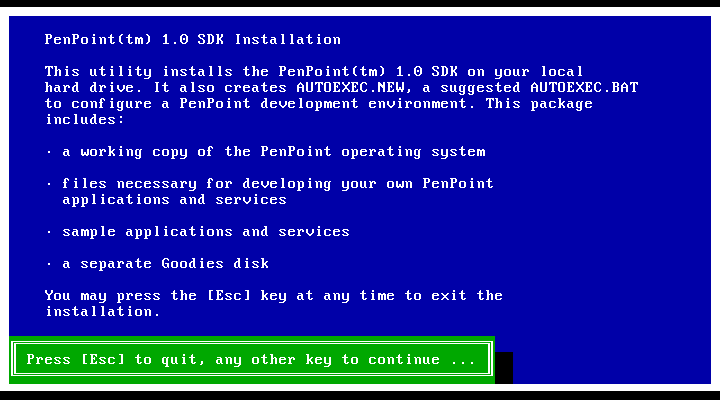
\includegraphics[width=\linewidth]{penpoint-installation-1.png}
        %\caption{PenPoint OS installation}
        %\label{fig:penpoint-installation-1}
    \end{subfigure}
    \hfill
    \begin{subfigure}[b]{0.45\linewidth}
        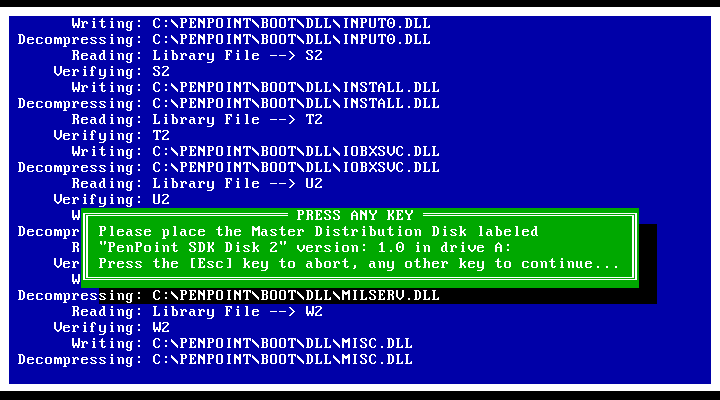
\includegraphics[width=\linewidth]{penpoint-installation-2.png}
        %\caption{PenPoint OS installation}
        %\label{fig:penpoint-instsallation-2}
    \end{subfigure}
    \caption{FreeDOS: PenPoint OS install wizard}
    \label{fig:penpoint-installation}
\end{figure}

Just before the installation wizard closes it informs that additional user
configuration will be required before running PenPointOS will be possible. It
tries to create or modify an existing \emph{CONFIG.SYS} file with a directive
\emph{FILES=20} and creates a new file called AUTOEXEC.NEW that has to be
incorporated into an existing \emph{AUTOEXEC.BAT} file
\ref{fig:penpoint-installation-2}.

\begin{figure}[H]
    \centering
    \begin{subfigure}[b]{0.45\linewidth}
        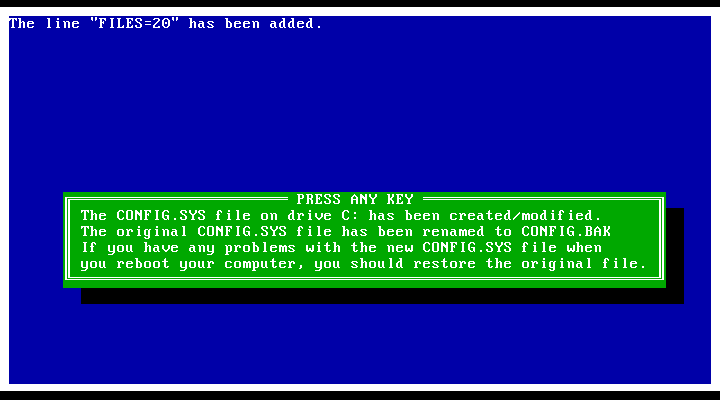
\includegraphics[width=\linewidth]{penpoint-installation-3.png}
        %\caption{PenPoint OS installation}
        %\label{fig:penpoint-installation-3}
    \end{subfigure}
    \hfill
    \begin{subfigure}[b]{0.45\linewidth}
        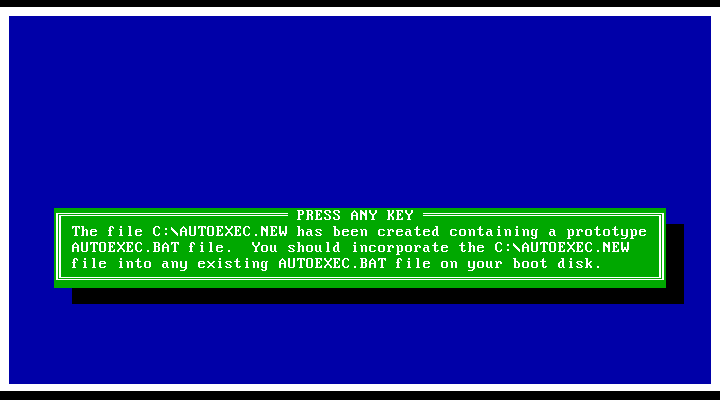
\includegraphics[width=\linewidth]{penpoint-installation-4.png}
        %\caption{PenPoint OS installation}
        %\label{fig:penpoint-instsallation-4}
    \end{subfigure}
    \caption{FreeDOS: PenPoint OS installation, config changes}
    \label{fig:penpoint-installation-2}
\end{figure}

FreeDOS actually by default uses \emph{FDCONF.SYS} and \emph{FDAUTO.BAT} files
instead. The config file is a special file that is run during startup and has
a special set of commands that can be run during boot. The \emph{FILES=20}
command sets the maximum number of file descriptors to 20. This is unnecessary
because default \emph{FDCONF.SYS} already uses a value of 40. The autoexec file
is a regular batch file that is automatically run after startup. The contents
of the \emph{AUTOEXEC.NEW} file are simply commands setting the environmental
variables used by PenPoint with paths from installation. These can be just
copied at the top of the \emph{FDAUTO.BAT} \ref{fig:fd-config}. It might be
useful to remember not to overwrite the \emph{PATH} variable but instead to
prepend the PenPoint value so that executables bundled with FreeDOS can still
be found.

\begin{figure}[H]
    \centering
    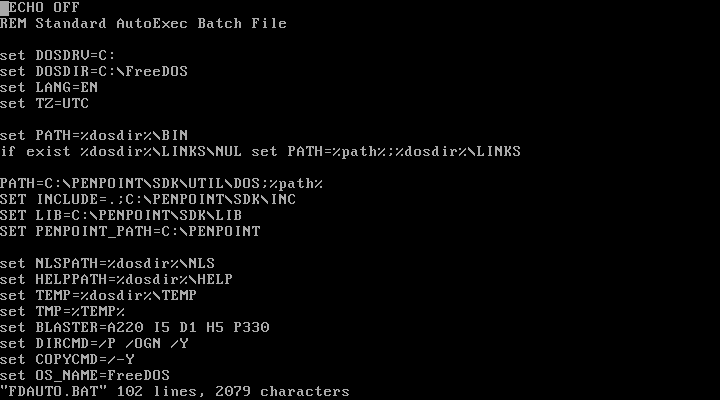
\includegraphics[width=0.9\linewidth]{fd-config.png}
    \caption{FreeDOS: FDAUTO.BAT config file}
    \label{fig:fd-config}
\end{figure}

Now we can try running PenPoint.

\subsection{Running PenPointOS}

%Now that the installation is complete to run PenPoint a script
%\emph{\\
%\textbackslash{}PENPOINT\textbackslash{}SDK\textbackslash{}UTIL\\
%\textbackslash{}DOS\textbackslash{}GO.BAT\\
%} \\
Now that the installation is complete to run PenPoint a script

\Verb[fontshape=it]|\PENPOINT\SDK\UTIL\DOS\GO.BAT|

\noindent
should be used. Here however we encounter the first problem. PenPoint does not
start, instead it crashes with a JemmEx exception \ref{fig:jemmex}.

\begin{figure}[H]
    \centering
    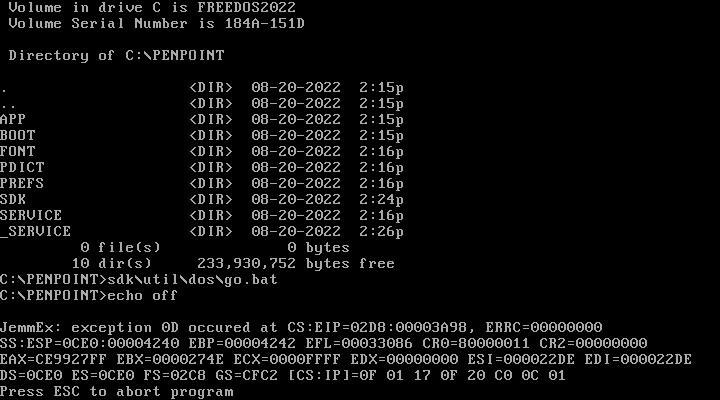
\includegraphics[width=0.9\linewidth]{jemmex.png}
    \caption{FreeDOS: JemmEx exception}
    \label{fig:jemmex}
\end{figure}

After trying a few things it turns out that this issue does not occur if FreeDOS
was booted in safe mode - one of the booting options defined in
\emph{FDCONF.SYS}. As it turns out JemmEx is in fact not loaded this way.
JemmEx is an Expanded Memory Manager. Expanded Memory was a workaround for 8088
and 8086 CPUs that allowed using the Upper Memory, that is between 640K and 1M
to address memory beyond 1M. Extended Memory on the other hand refers to memory
beyond the 1M on 286 and newer processors which could address this memory
normally. PenPointOS does not support Expanded Memory and only works on Extended
Memory \cite{godevtools}.

Now after removing loading JemmEx from startup PenPointOS starts. However there
is another problem. After some loading a broken pen and a number 1000 appears,
and the initialisation hangs \ref{fig:broken-pen}.

\begin{figure}[H]
    \centering
    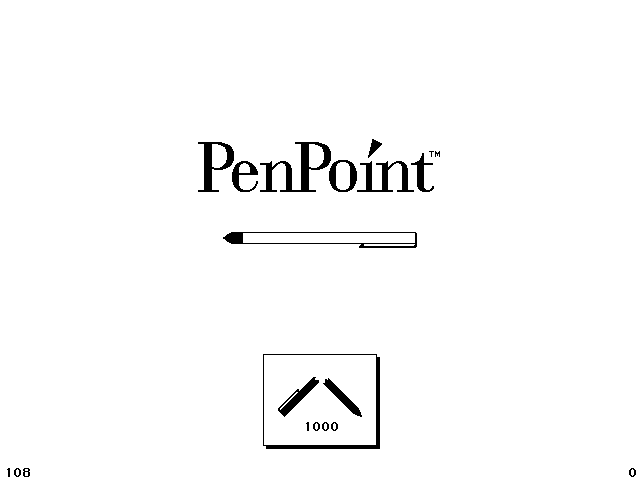
\includegraphics[width=0.9\linewidth]{broken-pen.png}
    \caption{PenPoint OS: broken pen error 1000}
    \label{fig:broken-pen}
\end{figure}

The error 1000 according to the ``Pen Point Development Tools'' book means that
no pointing device was enabled in the \emph{MIL.INI} file \cite{godevtools}.
After uncommenting the line that enables PS2 mouse support in \emph{MIL.INI}
\ref{fig:mil-ini}, PenPointOS boots correctly \ref{fig:penpoint-mainscreen}.

\begin{figure}[H]
    \centering
    \begin{subfigure}[b]{0.45\linewidth}
        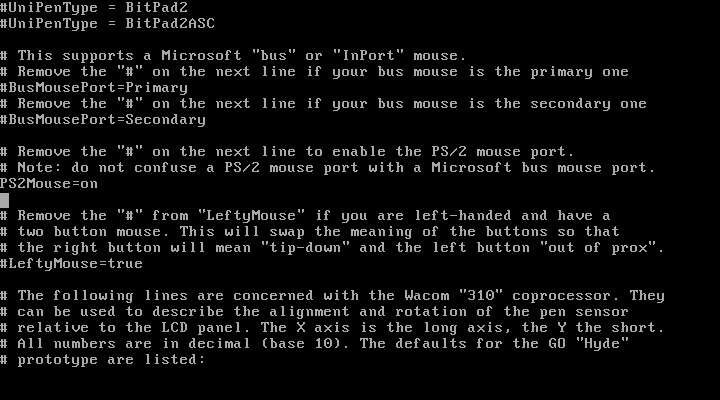
\includegraphics[width=\linewidth]{mil-ini.png}
        \caption{FreeDOS: MIL.INI}
        \label{fig:mil-ini}
    \end{subfigure}
    \hfill
    \begin{subfigure}[b]{0.45\linewidth}
        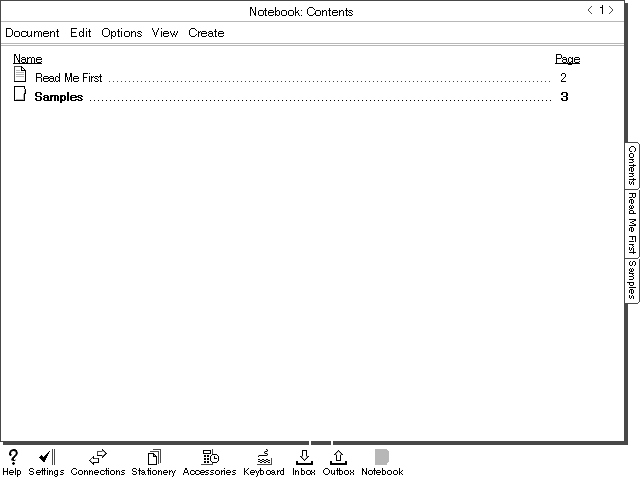
\includegraphics[width=\linewidth]{penpoint-mainscreen.png}
        \caption{PenPoint OS: main screen}
        \label{fig:penpoint-mainscreen}
    \end{subfigure}
    \caption{booted PenPoint OS}
\end{figure}

\subsection{Using a graphics tablet to point}

Now PenPoint is running and working correctly with a mouse.  Unfortunately just
because a mouse is working does not mean that other pointing devices will work
as well.  For example a mouse and a graphics tablet used with a finger work
without issue, but using a stylus is unwieldy.  Instead of moving with the pen
on the tablet, the pointer behaves more like a joystick - when the stylus is in
the middle of the tablet the pointer is stationary but when stylus is moved off
centre then the pointer moves in that direction, and the farther the stylus is
from the centre the faster it moves.  All of this happens because a mouse or
a finger movement on a tablet is a relative movement - the mouse moves by some
distance in a direction then the pointer should also move by that distance in
that direction, a stylus or a touchscreen, on the other hand, use absolute
movement - the stylus touches one corner of the tablet, the pointer should be
moved to the coroner of the screen.  The PS2 mouse emulation QEMU provides does
not have this functionality.

% TODO: \dots?
\begin{codeblock}
    \lstinputlisting[
        caption=ps2.c,
        language=C++,
        linerange={783-785,793-794,802-810,835-836},
    ]{ps2-old.c}
\end{codeblock}
%\begin{minipage}{\linewidth}
%    \begin{addmargin}[8mm]{0mm}
%        \begin{lstlisting}[
%            language=C++,
%            numbers=left,
%            firstnumber=1,
%            %    caption={\emph{Hello world} w HTML},
%            aboveskip=10pt,
%            %escapeinside=``,
%            breaklines=true,
%            ]
%static void ps2_mouse_event(DeviceState *dev, QemuConsole *src,
%                            InputEvent *evt)
%{
%    ...
%    PS2MouseState *s = (PS2MouseState *)dev;
%    InputMoveEvent *move;
%    ...
%
%    switch (evt->type) {
%    case INPUT_EVENT_KIND_REL:
%        move = evt->u.rel.data;
%        if (move->axis == INPUT_AXIS_X) {
%            s->mouse_dx += move->value;
%        } else if (move->axis == INPUT_AXIS_Y) {
%            s->mouse_dy -= move->value;
%        }
%        break;
%    ... 
%    }
%}
%        \end{lstlisting}
%    \end{addmargin}
%\end{minipage}

%QEMU also provides a graphics tablet emulation but it is a USB HID device that
%has to be initialised by the operating system. Simply adding a case handling an
%absolute movement to the PS2 mouse code, similar to the one in the source of
%the HID device, makes the mouse stop working altogether. It would probably have
%to keep a state where the pointer is and calculate the delta from there.
%
%
%\begin{minipage}{\linewidth}
%    \begin{addmargin}[8mm]{0mm}
%        \begin{lstlisting}[
%            language=C++,
%            numbers=left,
%            firstnumber=1,
%            %    caption={\emph{Hello world} w HTML},
%            aboveskip=10pt
%            ]
%    case INPUT_EVENT_KIND_ABS:
%        move = evt->u.abs.data;
%        if (move->axis == INPUT_AXIS_X) {
%            s->mouse_dx = move->value;
%        } else if (move->axis == INPUT_AXIS_Y) {
%            s->mouse_dy = move->value;
%        }
%        break;
%        \end{lstlisting}
%    \end{addmargin}
%\end{minipage}

%At this point in time it is impossible to get rid of this issue without a big
%time investment. 

%Fortunately u
Using both a mouse and a tablet works out of the box in a different
virtual machine program: VirtualBox. VirtualBox follows a more plug-and-play
philosophy at a cost of being generally slower than QEMU. It has much less
configuration options, is less optimised and does not provide support for such
functionality as using devices directly with passthrough. The developers of
VirtualBox have put an effort into it working without the need for much
configuration instead.% The incurred speed penalty from using VirtualBox and not
%QEMU to run PenPoint is not perceivable if it is there at all.




\clearpage % Rozdziały zaczynamy od nowej strony.

\section{Making tablet and stylus work in FreeDOS in QEMU}

% hid nie działa bo nie ma go kto zainicializować
% in the following section...

QEMU supports using tablet as a pointing device but it does not work in FreeDOS
because QEMU only provides a generic Human Interface Device (HID) driver.  The
USB-HID specification is a standard that allows for many different input and
output devices to communicate with the computer without any additional software.
For the QEMU HID device to work however it must be initialised by the operating
system.  DOS obviously came long before HID standard was created, and so it is
not supported by FreeDOS.

In this section I will describe the process of making the tablet behave as the
pointing device in the expected way inside FreeDOS on QEMU.

\subsection{Creating testing environment}

% używanie qemu bez trzymanki trudne

QEMU is extremely feature rich.  This is a great advantage, however it makes
using, tuning configuring it pretty cumbersome, especially since QEMU by itself
only provides console arguments as a way to specify settings.

\subsubsection{libvirt}

% co to libvirt, virsh, virt-manager

Libvirt is a collection of software whose goal is to provide simple, continent
and unified way to manage virtualisation functionality such as virtual machines
and hypervisors, but also containers and network interfaces.  The pieces of
software that make up libvirt are a stable C API, a libvirtd daemon, and
a command line client virsh.

But virsh is not the only client.  The way libvirt operates anyone can use the
API to communicate with the daemon in their client.  Apart from virsh GOME
provides its own libvirt client - GOME Boxes - that matches the rest of their
environment, and there also exist an add-on to cockpit - the web-based server
administration tool.  I used virt-manager.

Here comes the problem however: although virt-manager proved to be great for
configuring amounts of memory, number of cores and adding peripherals, it does
not allow a way to change the path of the used QEMU executable, and overwriting
an executable provided and managed by the distribution's package manager is
something that could lead to serious issues.

\subsubsection{Using virsh}

% virsh dump cmd: zrzut
% virsh edit: zrzut
% sprawdzanie logów: zrzut

My first thought was to somehow find out the exact way that virt-manager
executes the QEMU binary, that is the command line parameters and maybe the
environment.  It turns out that every guest configuration is stored in xml
format in something called the domain.  It also turns out that the virsh command
line libvirt client has the ability to convert that xml to equivalent shell
invocation.

\begin{codeblock}
    \dots
    \lstinputlisting[
        caption={},
        language=bash,
        linerange={7-15},
        deletekeywords={local,wait},
    ]{virsh-domxml-to-native.sh}
    \dots
    \lstinputlisting[
        caption={},
        language=bash,
        linerange={29-36},
        deletekeywords={local,wait},
    ]{virsh-domxml-to-native.sh}
    \dots
    \lstinputlisting[
        caption={\lstinline|virsh domxml-to-native qemu-argv --domain PenPointOS|},
        language=bash,
        linerange={56-59},
        deletekeywords={local,wait},
    ]{virsh-domxml-to-native.sh}
\end{codeblock}

This however still did not work.  At the very least many of the paths for files
and directories that it used for example in the \lstinline{/var/lib/libvirt} are
dynamically created at runtime.  I tried copying them and adjusting the startup
script accordingly but it still would not cooperate.  This clearly was not the
right approach.

How about modifying the domain xml directly?  Fortunately virsh allows to do
this using the \emph{edit} command.

\begin{codeblock}
    \lstinputlisting[
        caption={},
        language=XML,
        linerange={1-16},
    ]{virsh-dumpxml.xml}

    \dots

    \lstinputlisting[
        caption={\lstinline|virsh edit PenPointOS|},
        language=XML,
        linerange={123-123},
    ]{virsh-dumpxml.xml}
\end{codeblock}

\noindent
Especially interesting is the line containing the \emph{emulator} tag.

\begin{codeblock}
    \lstinputlisting[
        caption={},
        language=XML,
        linerange={35-36},
    ]{virsh-dumpxml.xml}
    
    \dots

    \lstinputlisting[
        caption={\lstinline|virsh edit PenPointOS|},
        language=XML,
        linerange={122-123},
    ]{virsh-dumpxml.xml}
\end{codeblock}

\noindent
According to libvirt documentation \cite{libvirt} the \emph{emulator} element
specifies the fully qualified path to the emulator binary.

With this knowledge I was able to clone the QEMU virtual machine which had
FreeDOS with PenPoint SDK installed and change the binary that was used for
emulation to the one supplied by me.  This way I could have two virtual machines
that differed only in the QEMU binary they used which was useful as
a comparison.

\subsection{Building QEMU} %?

% info z aur
% configure
% make depends
% brak spice-protocol

When using QEMU in conjunction with other tools like libvirt it is important
that it is built with all the required functionality.  QEMU uses
a \emph{configure} script to determine local build environment characteristic.
One way to increase the build speed is to configure the build environment to
only compile the x86 system target.

\begin{codeblock}
    \begin{lstlisting}[
        caption={configure},
        language=bash,
        numbers=none,
        deletekeywords={enable},
    ]
        ../configure \
            --target-list=x86_64-softmmu \
            --sysconfdir=/etc --localstatedir=/var \
            --libexecdir=/usr/lib/qemu --smbd=/usr/bin/smbd \
            --enable-modules --enable-sdl --disable-werror
    \end{lstlisting}
\end{codeblock}

The \emph{virsh edit} command verifies correctness of the modified domain
configuration.  In my case it was able to detect that the newly built QEMU
binary was missing support for SPICE which virt-manager used for display and
input to that virtual machine.  A good way to find out how QEMU must be
configured and its dependencies is to inspect how a package for specified system
is built.  On Arch Linux one can easily read \emph{PKGBUILD} - a file describing
the build process - for \emph{qemu-git} on Arch User Repository.

\subsection{Changes to QEMU source code}

% możliwość użycia tabletu w ppos, brak dokumentów itp.
% użycie ps2 do emulowania myszy
% opis ps2?
% centrum jest ui/input.c
%   w jaki sposób przekazuje info, skąd bierze, skąd wiadomo czy abs czy rel
% w moim przypadku dostaje info z ui/spice
% kod ps2

Although PenPoint supports multiple tablet devices, and even provides an option
to define a communication protocol for unsupported one \cite{godevtools}, I was
not able to find any information about graphical tablets from that time, much
less technical documentation that would be needed to create emulated version.

This however is not necessary.  Instead of creating a new device, a device that
is already present in QEMU and whose protocol is well supported - the PS/2
mouse.  That is how Synaptic touchpad worked: when Synaptic drives that
supported absolute mode were not present the touchpad identified itself as
a mouse and used either PS/2, Serial or Apple Desktop Bus protocols
\cite{synapticsinterfacing}.

\subsubsection{PS/2 protocol}

Although the PS/2 protocol was introduced by IBM in 1987 the port was still
present on most of the desktop motherboards sold until just few years ago.
Over the years many extensions of the standard were created by the likes of

Logitech or Microsoft.
One such popular extensions is the Microsoft Intellimouse extensions which
allowed for use of scroll wheel or scroll wheel and five buttons instead of the
usual three \cite{ps2interface}.

Normally the PS/2 mouse sends information about its movement in a packet of
three bytes \ref{table:ps2packet3b}.

\begin{table}[H]
    \begin{tabular}{lllllllll}
        & bit 7 & bit 6 & bit 5 & bit 4 & bit 3 & bit 2 & bit 1 & bit 0 \\

        \cline{2-9} 

        \multicolumn{1}{l|}{byte 1}        & \multicolumn{1}{l|}{Y overflow}   &
        \multicolumn{1}{l|}{X overflow}    & \multicolumn{1}{l|}{Y sign}       &
        \multicolumn{1}{l|}{X sign}        & \multicolumn{1}{l|}{always 1}     &
        \multicolumn{1}{l|}{M btn} & \multicolumn{1}{l|}{R btn} &
        \multicolumn{1}{l|}{L btn} \\

        \cline{2-9} 

        \multicolumn{1}{l|}{byte 2} & \multicolumn{8}{c|}{X movement} \\

        \cline{2-9} 

        \multicolumn{1}{l|}{byte 3} & \multicolumn{8}{c|}{Y movement} \\

        \cline{2-9} 
    \end{tabular}
    \caption{PS/2 mouse packet \cite{ps2interface}}
    \label{table:ps2packet3b}
\end{table}

\noindent
In order to enable the Intellimouse extensions the mouse sends a sequence of
three `Set sample rate' commands with predefined magic values.  A driver
compatible with that extension replies by issuing a `Get device ID' command to
which the mouse will respond with ID of 0x03.  Now both devices switch to using
four byte packets \ref{table:imps2scroll} \ref{table:imps25buttons}.

\begin{table}[H]
    \begin{tabular}{lllllllll}
        & bit 7 & bit 6 & bit 5 & bit 4 & bit 3 & bit 2 & bit 1 & bit 0 \\

        \cline{2-9} 

        \multicolumn{1}{l|}{byte 1}        & \multicolumn{1}{l|}{Y overflow}   &
        \multicolumn{1}{l|}{X overflow}    & \multicolumn{1}{l|}{Y sign}       &
        \multicolumn{1}{l|}{X sign}        & \multicolumn{1}{l|}{always 1}     &
        \multicolumn{1}{l|}{M btn} & \multicolumn{1}{l|}{R btn} &
        \multicolumn{1}{l|}{L btn} \\

        \cline{2-9} 

        \multicolumn{1}{l|}{byte 2} & \multicolumn{8}{c|}{X movement} \\

        \cline{2-9} 

        \multicolumn{1}{l|}{byte 3} & \multicolumn{8}{c|}{Y movement} \\

        \cline{2-9} 

        \multicolumn{1}{l|}{byte 4} & \multicolumn{8}{c|}{Z movement} \\

        \cline{2-9} 
    \end{tabular}
    \caption{Intellimouse PS/2 mouse with scroll wheel packet \cite{ps2interface}}
    \label{table:imps2scroll}
\end{table}

\noindent
and

\begin{table}[H]
    \begin{tabular}{lllllllll}
        & bit 7 & bit 6 & bit 5 & bit 4 & bit 3 & bit 2 & bit 1 & bit 0 \\

        \cline{2-9} 

        \multicolumn{1}{l|}{byte 1}     & \multicolumn{1}{l|}{Y overflow}   &
        \multicolumn{1}{l|}{X overflow} & \multicolumn{1}{l|}{Y sign}       &
        \multicolumn{1}{l|}{X sign}     & \multicolumn{1}{l|}{always 1}     &
        \multicolumn{1}{l|}{M btn}      & \multicolumn{1}{l|}{R btn}        &
        \multicolumn{1}{l|}{L btn} \\

        \cline{2-9} 

        \multicolumn{1}{l|}{byte 2} & \multicolumn{8}{c|}{X movement} \\

        \cline{2-9} 

        \multicolumn{1}{l|}{byte 3} & \multicolumn{8}{c|}{Y movement} \\

        \cline{2-9} 

        \multicolumn{1}{l|}{byte 4}     & \multicolumn{2}{c|}{always 0} &
        \multicolumn{1}{l|}{5th btn}    & \multicolumn{1}{l|}{4th btn}  &
        \multicolumn{4}{c|}{Z movement} \\

        \cline{2-9} 
    \end{tabular}
    \caption{Intellimouse PS/2 mouse with scroll wheel + 5 buttons packet \cite{ps2interface}}
    \label{table:imps25buttons}
\end{table}

\noindent
The QEMU PS/2 mouse device supports both of these extensions.

There does not seem to be any current publication of the standard
\cite{ps2interface}.

\subsubsection{SPICE initialization}

SPICE project is a software solution that aims to provide remote-display to
virtual environments, on the same computer or anywhere on the internet.  It is
comprised of the SPICE protocol, server, and several client implementations are
available.  The \emph{virt-manager} program uses either SPICE or VNC to provide
display and pointer input, and QEMU is compatible also with other sources.  The
description of SPICE is ilustratory. % TODO

QEMU defines a SPICE module.

\begin{codeblock}
    \lstinputlisting[
        caption=spice-core.c,
        language=C,
        linerange={968-985},
    ]{spice-core.c}
\end{codeblock}

Inside the \emph{qemu\_spice\_init} function \emph{qemu\_spice\_input\_init}
function is called.

\begin{codeblock}
    \lstinputlisting[
        caption={},
        language=C,
        linerange={640-641},
    ]{spice-core.c}
    \dots
    \lstinputlisting[
        caption={},
        language=C,
        linerange={827-827},
    ]{spice-core.c}
    \dots
    \lstinputlisting[
        caption=spice-core.c,
        language=C,
        linerange={852-852},
    ]{spice-core.c}
\end{codeblock}

The \emph{qemu\_spice\_input\_init} function adds the keyboard and mouse
interfaces, and adds and calls a mouse mode notifier.

\begin{codeblock}
    \lstinputlisting[
        caption=spice-input.c,
        language=C,
        linerange={243-262},
    ]{spice-input.c}
\end{codeblock}

The \emph{mouse\_mode\_notifier} adds a SPICE tablet interface if there is an
input handler with absolute mode available.

\begin{codeblock}
    \lstinputlisting[
        caption=spice-input.c,
        language=C,
        linerange={226-241},
    ]{spice-input.c}
\end{codeblock}

The function \emph{qemu\_input\_is\_absolute} simply checks if any of the
registered input handlers has the \emph{INPUT\_EVENT\_MASK\_ABS} flag set.

\begin{codeblock}
    \lstinputlisting[
        caption=input.c,
        language=C,
        linerange={493-500},
    ]{input.c}
\end{codeblock}

\subsubsection{PS/2 input device initialization}

The QEMU PS/2 mouse is registered using the standard QEMU interface for adding
devices.

% static const TypeInfo ps2_mouse_info
% ps2_info 
% ps2_register_types
% type_init
\begin{codeblock}
    \lstinputlisting[
        caption={ps2.c},
        language=C,
        linerange={1309-1315,1331-1339,1341-1346,1348-1348},
    ]{ps2-new.c}
\end{codeblock}

The \emph{ps2\_info} is used as a base type for both PS/2 mouse and keyboard.
Inside the PS/2 mouse class initialization function a realization function is
set to register the PS/2 mouse device as an input handler.

% ps2_mouse_realize
% ps2_mouse_class_init
\begin{codeblock}
    \lstinputlisting[
        caption={ps2.c},
        language=C,
        linerange={1276-1279,1298-1307},
    ]{ps2-new.c}
\end{codeblock}

\noindent
The reset function sets all of the device state to the initial values, and the
VM state description structure is used to provide a mechanism to save and
restore the state of all devices.

The \emph{qemu\_input\_handler\_register} function is called with a struct that
describes the capabilities of the mouse and callbacks for events and syncing.
Here the \emph{INPUT\_EVENT\_MASK\_ABS} is added to indicate that the PS/2 mouse
can work in absolute mode.  Setting this flag will make it so that the SPICE
tablet interface is added, and absolute mode events will be handled by the PS/2
mouse device.

% ps2_mouse_handler
\begin{codeblock}
    \lstinputlisting[
        caption=ps2.c,
        language=C,
        linerange={1269-1279},
    ]{ps2-new.c}
\end{codeblock}

\subsubsection{How input in QEMU is processed}

When pointer position changes SPICE uses either mouse or tablet interfaces that
were initialised in the \emph{qemu\_spice\_input\_init} function.  If absolute
input handler is available the tablet interface is used for absolute pointer
% TODO czy tylko?
position changes.

\begin{codeblock}
    \lstinputlisting[
        caption=spice-input.c,
        language=C,
        linerange={215-224},
    ]{spice-input.c}
\end{codeblock}

SPICE calls the \emph{tablet\_position} function using the \emph{position}
member of the tablet interface.

\begin{codeblock}
    \lstinputlisting[
        caption=spice-input.c,
        language=C,
        linerange={184-194},
    ]{spice-input.c}
\end{codeblock}

The \emph{tablet\_position} queues the absolute input for both axes and issues
the event sync.

The \emph{qemu\_input\_queue\_abs} scales the input value and sends the event.
The \emph{qemu\_input\_send\_event} function performs some checks and calls the
\emph{replay\_input\_event}, which adds the event to replay if in replay mode,
and otherwise it calls the \emph{qemu\_input\_send\_event\_impl}.  Finally this
function finds an appropriate input handler and calls its event callback.

\begin{codeblock}
    \lstinputlisting[
        caption={},
        language=C,
        linerange={529-543},
    ]{input.c}
    \lstinputlisting[
        caption={},
        language=C,
        linerange={353-354,378-379},
    ]{input.c}
    \lstinputlisting[
        caption=input.c,
        language=C,
        linerange={333-334,345-351},
    ]{input.c}
\end{codeblock}

\noindent
The event sync functionality is implemented similarly ending in calling the
input handler callback for syncing.

\subsubsection{Emulation of absolute input using PS/2 mouse device}

Because the PS/2 mouse protocol uses relative pointer mode - that is it
transfers by how much the mouse moved from the last position - and a tablet
provides values in absolute mode - that is it reports the current absolute
stylus position - the absolute mode values must be converted to relative terms
somehow.  To do so the mouse device structure should hold the last known
absolute position.  Whenever an event occurs the last known absolute position
would be updated, and when handling an event with absolute movement the position
difference could be calculated and communicated using the standard PS/2
protocol.

The fields \emph{absolute\_x} and \emph{absolute\_y} are added to the
\emph{PS2MouseState} structure.

%\begin{codeblock}
%    \begin{lstlisting}[
%        caption=ps2.h,
%        language=C,
%        escapechar=!,
%    ]
%struct PS2MouseState {
%    PS2State parent_obj;
%
%    uint8_t mouse_status;
%    uint8_t mouse_resolution;
%    uint8_t mouse_sample_rate;
%    uint8_t mouse_wrap;
%    uint8_t mouse_type; /* 0 = PS2, 3 = IMPS/2, 4 = IMEX */
%    uint8_t mouse_detect_state;
%    int mouse_dx; /* current values, needed for 'poll' mode */
%    int mouse_dy;
%    int mouse_dz;
%    int mouse_dw;
%    !\colorbox{green}{{int absolute\_x;}}!
%    !\colorbox{green}{{int absolute\_y;}}!
%    uint8_t mouse_buttons;
%};
%    \end{lstlisting}
%\end{codeblock}

\begin{codeblock}
    \lstinputlisting[
        caption=ps2.h,
        language=C,
        linerange={81-97},
    ]{ps2-new.h}
\end{codeblock}

They are also added to the reset function, and the \emph{VMStateDescription}
struct.

\begin{codeblock}
    \lstinputlisting[
        caption=ps2.c,
        language=C,
        linerange={1091-1112,1114-1126}
    ]{ps2-new.c}
\end{codeblock}

The \emph{INPUT\_EVENT\_MASK\_ABS} flag is also set for the PS/2 mouse input
handler.  This makes it so that QEMU recognizes that it can handle absolute
input, and that SPICE registers the tablet interface.  Then events with absolute
movement are sent to the PS/2 mouse input handler \emph{event} function.

\begin{codeblock}
    \lstinputlisting[
        caption=ps2.c,
        language=C,
        linerange={1269-1274},
    ]{ps2-new.c}
\end{codeblock}

Finally the code that updates the current known absolute position, and
calculates the absolute movement deltas is added to the \emph{ps2\_mouse\_event}
function.

\begin{codeblock}
    \lstinputlisting[
        caption=ps2.c,
        language=C,
        linerange={783-785,802-848,873-874},
    ]{ps2-new.c}
\end{codeblock}




% TODO poprawić conclusion/further works


\clearpage % Rozdziały zaczynamy od nowej strony.

%\section{Summary}
\section{Summary and conclusions}

The goal of this work was to run PenPoint OS on a modern computer with
reasonable performance, and be able to use it with the help of a mouse,
a graphics tablet or a touchscreen. PenPoint was an important and influential
albeit now mostly forgotten piece of computing history. It is important to
preserve it and at the same time maybe gain a little insight.

%The first approach consisted of trying to port modifications of the JPC
%emulator created by professor Simon Schubiger to the QEMU hypervisor. The JPC
%emulator was not performant enough to run PenPoint OS at a speed that would be
%comfortable to use. First the changes to the JPC emulator required to run
%PenPoint were discussed in detail: what they do, how they do it, and how all of
%this relates to the general architecture of the JPC. Then the operation of the
%QEMU hypervisor, the process of defining a new device in the QEMU source tree
%and making it available to QEMU, and the reasoning behind choosing QEMU were
%described in depth. This approach however was abandoned because of the
%complexity and because an easier way became available.

The first approach consisted of trying to port modifications of the JPC
emulator created by professor Simon Schubiger to the QEMU hypervisor.  The JPC
emulator was not performant enough to run PenPoint OS at a speed that would be
comfortable to use.  First the changes to the JPC emulator required to run
PenPoint were discussed in detail: what they do, how they do it, and how all of
this relates to the general architecture of the JPC.  Then the operation of the
QEMU hypervisor, the process of defining a new device in the QEMU source tree
and making it available to QEMU, and the reasoning behind choosing QEMU were
described in depth.  This approach however was abandoned because it was deemed
unnecessarily complex, and outside of the scope of this work.  Instead a more
straightforward and less error prone solution was chosen.

\begin{figure}[!h]
    \centering
    \includegraphics[width=0.9\linewidth]{penpoint-pc-tablet.png}
    \caption{PenPoint OS running on PC with a graphics tablet}
    \label{fig:penpoint-pc-tablet}
\end{figure}

In the second approach a different distribution of PenPoint OS was used, one
that was created so that it could be installed on a PC running MS-DOS.  Here the
process of obtaining the installation files, the installation, and configuration
of the DOS environment created using FreeDOS, and of PenPoint is described.
First it was described how the SDK distribution of PenPoint differs from the
version created for the NCR 3125.  Then it was shown how the floppy disk files
ought to be prepared to be used with a virtual machine, and the process of
installation was explained.  Finally it was demonstrated how to configure the
FreeDOS environment to run PenPoint OS and how to configure PenPoint OS itself
to work with a mouse.  The difference between a relative and absolute pointing
device was discussed as well.  Finally the process of handling mouse and tablet
input in QEMU was described, as well as the implementation of adding the
absolute pointing mode functionality, and how the conversion from absolute
values to relative values is performed in the PS/2 mouse QEMU device.

%, how it works in both QEMU and VirtualBox, and what
%was tried and what should be done in QEMU to support an absolute pointing device
%like a graphics tablet.

% conclusions
The original goal of running PenPoint OS on modern hardware was met
\ref{fig:penpoint-pc-tablet} by using the SDK distribution of PenPoint and
installing it on FreeDOS in a modified version of QEMU.

\begin{itemize}
    \item
        It is possible to run PenPoint on any computer that can run QEMU
    \item
        The performance of this solution is excellent
    \item
        It is possible to use a graphics tablet or a touch screen as a pointing
        device
\end{itemize}

%Potential improvements include modifying source code of QEMU so that absolute
%pointing methods work with it correctly, and porting the changes to JPC
%emulator created by professor Schubiger to either VirtualBox or QEMU to run the
%PenPoint OS version for NCR System 3125 - the flagship PenPoint device - with
%all of its bells and whistles.

Potential improvements include creating a QEMU device that would represent
a graphical tablet from the era.  This would not change the functionality of the
of the solution but it would be more `authentic' and complete.  Modifying QEMU
to run the NCR 3125 version of PenPoint instead of the developer version could
also prove beneficial, as it was the flagship PenPoint device that offered THE
experience that creators of PenPoint intended.  It could also be useful to use
outside of PenPoint of other software that was created for System 3125.



%\clearpage % Rozdziały zaczynamy od nowej strony.

\section{Conclusions and further work}

The original goal of running PenPoint OS on modern hardware was met by using
the SDK distribution of PenPoint and installing it on FreeDOS in VirtualBox:

\begin{itemize}
    \item
        It is possible to run PenPoint on any computer that can run VirtualBox
    \item
        The performance of this solution is excellent
    \item
        It is possible to use a graphics tablet or a touch screen as a pointing
        device
\end{itemize}

Potential improvements include modifying source code of QEMU so that absolute
pointing methods work with it correctly, and porting the changes to JPC
emulator created by professor Schubiger to either VirtualBox or QEMU to run the
PenPoint OS version for NCR System 3125 - the flagship PenPoint device - with
all of its bells and whistles.



%---------------
% Bibliografia
%---------------
\cleardoublepage % Zaczynamy od nieparzystej strony
\printbibliography
\clearpage

% Wykaz symboli i skrótów.
% Pamiętaj, żeby posortować symbole alfabetycznie
% we własnym zakresie. Makro \acronymlist
% generuje właściwy tytuł sekcji, w zależności od języka.
% Makro \acronym dodaje skrót/symbol do listy,
% zapewniając podstawowe formatowanie.
% TODO
%\acronymlist
%\acronym{EiTI}{Wydział Elektroniki i Technik Informacyjnych}
%\acronym{PW}{Politechnika Warszawska}
%\acronym{WEIRD}{ang. \emph{Western, Educated, Industrialized, Rich and Democratic}}
\vspace{0.8cm}

%--------------------------------------
% Spisy: rysunków, tabel, załączników
%--------------------------------------
\pagestyle{plain}

\listoffigurestoc    % Spis rysunków.
%\vspace{1cm}         % vertical space
%\listoftablestoc     % Spis tabel.
%\vspace{1cm}         % vertical space
%\listofappendicestoc % Spis załączników

%-------------
% Załączniki
%-------------

% Obrazki i tabele w załącznikach nie trafiają do spisów
\captionsetup[figure]{list=no}
\captionsetup[table]{list=no}

%% Załącznik 1
%\clearpage
%\appendix{Nazwa załącznika 1}
%\lipsum[1-3]
%\begin{figure}[!h]
%	\centering \includegraphics[width=0.5\linewidth]{logopw2.png}
%	\caption{Obrazek w załączniku.}
%\end{figure}
%\lipsum[4-7]
%
%% Załącznik 2
%\clearpage
%\appendix{Nazwa załącznika 2}
%\lipsum[1-2]
%\begin{table}[!h] \centering
%    \caption{Tabela w załączniku.}
%    \begin{tabular} {| c | c | r |} \hline
%        Kolumna 1       & Kolumna 2 & Liczba \\ \hline\hline
%        cell1           & cell2     & 60     \\ \hline
%        \multicolumn{2}{|r|}{Suma:} & 123,45 \\ \hline
%    \end{tabular}
%\end{table}
%\lipsum[3-4]

% Używając powyższych spisów jako szablonu,
% możesz dodać również swój własny wykaz,
% np. spis algorytmów.

\end{document} % Dobranoc.
